\documentclass{article}
\usepackage{anyfontsize}
\usepackage{graphicx}
\usepackage{hyperref}
\usepackage{parskip}
\usepackage{enumitem}
\usepackage{array}
\usepackage{tabularx}
\usepackage[section]{placeins}
\usepackage{float}% If comment this, figure moves to Page 2
\usepackage[dvipsnames]{xcolor}
\usepackage{listings}
\usepackage{alloy-style}

\fontsize{10pt}{12pt}\selectfont % Set the font size
\begin{document}

% FRONT PAGE
\begin{titlepage}
    \begin{center}
        
        Politecnico di Milano\\
      
        Computer Science and Engineering\\
        
        Software Engineering II\\

        \vfill
        
        {\Large \textbf{RASD - CodeKataBlade}}\\
        
        \vfill

        José Alejandro Sarmiento

        \today

        v1.0
        
    \end{center}
\end{titlepage}
\newpage


% TABLE OF CONTENTS
\tableofcontents


\section{INTRODUCTION}
\subsection{Purpose}

The primary purpose of the CodeKataBattle (CKB) platform is to provide an environment 
for students to enhance their software development skills through collaborative 
learning and competition, and for educators to set up these scenarios. The platform facilitates 
this by allowing educators to setup tournaments where code kata battles are organized.

\textbf{A) Skill Enhancement through Practice:}

CKB serves as a virtual arena where students can test and improve their programming abilities by actively 
participating in code kata battles.

\textbf{B) Educator-Guided Learning:}

The platform must allow for educators to create tournaments, compose battles and perform manual evaluations
on top of automated ones. This ensures that the learning experience aligns with the curriculum and instructional goals.

\textbf{C) Automated Evaluation:}

CKB should have an automated evaluation system that provides feedback to students based on
 objective criteria. Specifically, the criteria the evaluation is based upon is the number of passed test cases 
 set up by the battle organizer and the timeliness. 

 \textbf{D) Competition and Recognition:}

The platform should have a leaderboard functionality that allows participants to 
gauge their performance and see how their skills compare to other participants.

In summary, CodeKataBattle aims to create a learning platform, combining 
hands-on coding practice, collaborative teamwork and automated feedback.

Knowing this, the S2B will have a certain set of goals to achieve:
\begin{itemize}
    \item \textbf{G1:} Every educator should be able to create a tournament.
    \item \textbf{G2:} When crearing a tournament, the educator doing so should be able to set a registration deadline and a name.
    \item \textbf{G3:} Every educator that owns a tournament should be able to invite other educators to it.
    \item \textbf{G4:} Every educator that belongs to a tournament should be able to create battles.
    \item \textbf{G5:} When creating a battle, the educator doing so should be able to set the programming language, a decription of the problem, the test cases which will evaluate the students code, the build automation scripts, the registration deadline, the final submission deadline, the minimum and maximum number of participants per group.
    \item \textbf{G6:} Every student should be able to see the list of tournaments and register to them before the registration deadline.
    \item \textbf{G7:} Every student should be able to see the description of the battles of a tournament they belong to and register to them before the registration deadline by themselves or with other students by inviting them to join or by accepting another student's invitation.
    \item \textbf{G8:} Every time a student makes a submission to a battle, the platform should evaluate it and update the leaderboard of the battle accordingly.
    \item \textbf{G9:} The evaluation carried on by the platform should be performed with the build automation scripts set by the educator and should be based on the test cases set by the educator and the timeliness of the submission.
    \item \textbf{G10:} Every student and educator should be able to see the leaderboard of a battle they belong to.
    \item \textbf{G11:} Once the battle ends, the educator that created it should be able to manually evaluate the code of the students if they so desire to and set a grade for each student.
    \item \textbf{G12:} Once the educator consolidates the results of a battle, the students that participated in it should be notified and the final results of the battle should be displayed to everyone. The leaderboard of the tournament the battle belongs to should be updated by adding for each student the battle score to the sum of all the other battles they have participated on.
    \item \textbf{G13:} Every student and educator should be able to see the leaderboard of every tournament.
    \item \textbf{G14:} An instructor that owns a tournament should be able to close it.
    \item \textbf{G15:} Once the owner of a tournament closes it, the platform should notify all the students once the leaderboard of the tournament is available.
    \item \textbf{G16:} When a tournament is created, all students should be notified. 
    \item \textbf{G17:} When a battle is created, all students participating in the tournament the battle belongs to should be notified.
    \item \textbf{G18:} A student should be able to browse the platform and find tournaments based on keywords like topics, educators' names, programming language and experience level.
    \item \textbf{G19:} A student should be able to cancel their registration to a tournament or battle before the registration deadline.

\end{itemize}

Goal G18 and G19 are not inferred from the description of the problem but it are goals that would be beneficial to the platform given its nature and certain situations that could occur.

\newpage

\subsection{Scope}  

The education sector in software development is an ever-growing field given the nature of the topic 
being teached. 

The CodeKataBattle (CKB) platform aims to provide a competitive twist to the learning
by facilitating the creation of competitions in the form of tournaments where students can showcase their abilities.

These are managed by educators who can create the aforementioned tournaments and compose battles where they can decide 
the programming language, the description of the problem and the test cases which will evaluate the students code among other things.

This way, through the use of GitHub, the platform can automatically evaluate the code of a team.

In the environment of the CodeKataBattle system the following actors are identified:

\textbf{Students:} These are the primary users of the CKB system. They participate in battles and tournaments to improve their software development skills. They can form teams, work on code katas, and submit their solutions.

\textbf{Educators:}: They are responsible for creating and managing battles and tournaments. They set various parameters for battles, evaluate the solutions submitted by students, and provide feedback.

\textbf{GitHub:} The CKB system integrates with GitHub for managing code kata projects and tracking students' commits. GitHub is a widely used platform for version control and collaboration in software development.

Having all of this in mind, the following are the World and Shared phenomena that the system will have to deal with:

\textbf{World Phenomena:}

\begin{itemize}
    \item \textbf{W1:} A group of students organizes themselves to participate in a battle together.
    \item \textbf{W2:} A group of students registered to a battle fork the repository of the battle.
    \item \textbf{W3:} Students set up an automated workflow through GitHub Actions that will notify the system every time a commit is pushed to the main branch of the forked repository of a battle.
    \item \textbf{W4:} A student pushes a commit to the main branche of a forked repository of a battle.
    \item \textbf{W5:} An educator possesses a specific evaluation criteria through which they perform their manual evaluations.
\end{itemize}

\textbf{Shared Phenomena:}

Controlled by the world and observed by the system.

\begin{itemize}
    \item \textbf{SP1:} An educator creates a tournament with a set of attributes.
    \item \textbf{SP2:} An educator creates a battle with a set of attributes inside a tournament.
    \item \textbf{SP3:} An educator invites other educators to a tournament.
    \item \textbf{SP4:} A student looks for a tournament.
    \item \textbf{SP5:} A student registers to a tournament.
    \item \textbf{SP6:} A student cancels a registration to a tournament.
    \item \textbf{SP7:} A student or a team of students registers to a battle.
    \item \textbf{SP8:} A student or a team of students cancels a registration to a battle.
    \item \textbf{SP9:} GitHub notfies the system that a student has pushed a commit to the main branch of a forked repository of a battle. 
    \item \textbf{SP10:} An educator performs manual evaluations on the submissions of a battle they own.
    \item \textbf{SP11:} An educator consolidates the results of a battle.
    \item \textbf{SP12:} An educator closes a tournament.
\end{itemize}

Controlled by the system and observed by the world.

\begin{itemize}
    \item \textbf{SP13:} The system notifies all the students that a tournament has been created.
    \item \textbf{SP14:} The system notifies all the students participating in a tournament that a battle has been created.
    \item \textbf{SP15:} The system displays the leaderboard of tournament while it is active and after it has ended.
    \item \textbf{SP16:} The system displays the leaderboard of a battle while it is active and after it has ended.
    \item \textbf{SP17:} The system updates a battle's leaderboard every time a new evaluation is performed.
    \item \textbf{SP18:} The system notifies all the students participating in a battle that the final results have been consolidated.
    \item \textbf{SP19:} The system updates the leaderboard of a tournament every time a battle ends.
    \item \textbf{SP20:} The system notifies all the students participating in a tournament that it has ended.
\end{itemize}

\newpage

\subsection{Definitions, Acronyms, Abbreviations}

\subsubsection{Definitions}
 
\begin{itemize}
    \item \textbf{Tournament:} A tournament is a space where educators can create battles and students can register to them. It has a registration deadline and a leaderboard that is updated every time a battle ends.
    \item \textbf{Battle:} A battle is a space where students can register to and submit their solutions to a problem. It has a registration deadline, a final submission deadline, a leaderboard that is updated every time a new evaluation is performed and a set of test cases that will be used to evaluate the submissions.
    \item \textbf{GitHub:} GitHub is a code hosting platform for version control and collaboration. It lets you and others work together on projects from anywhere.
    \item \textbf{GitHub Actions:} GitHub Actions is a CI/CD tool that allows you to automate your software development workflows in the same place you store code and collaborate on pull requests and issues.
    \item \textbf{Educator:} An educator, in the context of the system, is a user of the platform that can create tournaments and battles, invite other educators to tournaments, perform manual evaluations on the submissions of a battle they own and consolidate the results of a battle.
    \item \textbf{Student:} A student, in the context of the system, is a user of the platform that can register to tournaments and battles, create teams and submit their solutions to a battle.
    \item \textbf{Build Automation Scripts:} Build automation scripts are scripts that are run automatically by the system every time a commit is pushed to the main branch of the forked repository of a battle. They are used to evaluate the submissions of the students.
    \item \textbf{Test Case:} A test case is a set of conditions under which a tester will determine whether an application, software system or one of its features is working as it was originally established for it to do.
    \item \textbf{Timeliness:} Timeliness is the quality of doing something or producing something at the right time. In the context of the system, it refers to the time in which a student submits their solution to a battle with respect to the start of the battle and the final submission deadline.
\end{itemize}

\subsubsection{Acronyms}

\begin{itemize}
    \item \textbf{CKB:} CodeKataBattle
    \item \textbf{S2B:} System to Be
    \item \textbf{TDD:} Test-Driven Development
    \item \textbf{CI/CD:} Continuous Integration/Continuous Delivery
    \item \textbf{UI:} User Interface
    \item \textbf{API:} Application Programming Interface
    \item \textbf{UML:} Unified Modeling Language
\end{itemize}

\subsubsection{Abbreviations}

\begin{itemize}
    \item \textbf{Gn:} Goal number n
    \item \textbf{Wn:} World Phenomena number n
    \item \textbf{SPn:} Shared Phenomena number n
    \item \textbf{Dn:} Domain Assumption number n
    \item \textbf{Rn:} Requirement number 
    \item \textbf{UCn:} Use Case number n
\end{itemize}


\subsection{Revision history}
v1,0 - 22/12/2023 - First release
\subsection{Reference Documents}

The specification of the RASD and DD assignment of the Software
Engineering II course, held by professor Matteo Rossi, Elisabetta Di Nitto and
Matteo Camilli at the Politecnico di Milano, A.Y 2023/2024;

\subsection{Document Structure}

\begin{itemize}
    \item \textbf{1. Introduction:} This section provides an overview of the entire document. It identifies the product’s goals and the scope of the system along with the definitions, acronyms, abbreviations and the revision history.
    \item \textbf{2. Overall Description:} This section provides a general description of the product and its functionality. It also describes the user characteristics, assumptions, dependencies and constraints.
    \item \textbf{3. Specific Requirements:} This section contains all the software requirements to a level of detail sufficient to enable designers to design a system to satisfy those requirements, and testers to test that the system satisfies those requirements.
    \item \textbf{4. Formal Analysis Using Alloy:} This section contains a formal analysis of the system using the Alloy language.
    \item \textbf{5. Effort Spent:} This section contains the number of hours each group member has worked on the document.
    \item \textbf{6. References:} This section contains all the reference documents used to create this document.
\end{itemize}

\section{OVERALL DESCRIPTION}
\subsection{Product perspective}
\subsubsection{Scenarios}

\begin{itemize}
    \item \textbf{1. Educator creates a tournament:} 
    
    An educator called Adam wants to create a tournament for his students. He goes to the CKB platform and creates a tournament with a registration deadline of 2 weeks from now. The platform notifies all the students that a tournament has been created. He then invites his colleagues to the tournament so when the tournament starts they can create battles.

    \textbf{Goals:} G1, G2, G3, G16.
    \textbf{Phenomena:} SP1, SP3, SP13.

    \item \textbf{2. Student registers to a tournament 1:}
    
    A student called Bob receives a notification that a tournament has been created by educator Adam. He goes to the CKB platform and registers to the tournament before the registration deadline.

    \textbf{Goals:} G6, G16.
    \textbf{Phenomena:} SP5, SP13.

    \item \textbf{5. Students registers to a tournament 2:}
    
    Francesca doesn't regularly check the notification the CKB platform sends her. She instead looks for tournaments by herself. Currently she considers herself an intermidiate level programmer in Java, so she uses the search functionality of the platform to find tournaments that have these characteristics. She then finds the tournament created by educator Charlie and registers to it. 

    \textbf{Goals:} G6, G16.
    \textbf{Phenomena:} SP4, SP5.
    
    \item \textbf{3. Educator creates a battle:}
    
    Educator Charlie wants to create a battle for the tournament he was invited to by educator Adam. He goes to the CKB platform and creates a battle with a registration deadline of 1 week from now, a final submission deadline of 2 weeks from now, a minimum of 1 participant per group and a maximum of 3 participants per group. He also sets the programming language to Java, the description of the problem and uploads the build automation scripts and test cases which will evaluate the students code. The platform notifies all the students participating in the tournament that a battle has been created.

    \textbf{Goals:} G4, G5, G17.
    \textbf{Phenomena:} SP2, SP14.

    \item \textbf{4. Students registers to a battle:}
    
    Bob receives a notification that a battle has been created by educator Charlie. He goes to the CKB platform and reads the description of the battle. He then contacts his friends Danielle and Eve, who are also inside educator Adam's tournament, and they decide to form a team and register to the battle together. Charlie invites Danielle and Eve to the battle and they accept. 

    \textbf{Goals:} G7, G17.
    \textbf{Phenomena:} W1, SP7, SP14.

    \item \textbf{5. Student cancels registration to battle:}
    
    Francesca wants to register to the battle set by educator Charlie with her friends Gabriel and Harry. She registers to the battle and invites them while doing so. However, Gabriel and Harry never accept the invitation. Francesca then decides to cancel her registration to the battle one day before the registration deadline expires. 

    \textbf{Goals:} G7, G19.
    \textbf{Phenomena:} W1, SP7, SP8, SP14.

    \item \textbf{5. Student submits a solution to a battle:}
    
    After the registrarion deadline ends, the system sends the link to the newly created GitHub repository to the students that registered to the battle. Bob, Danielle and Eve fork the repository and set up an automated workflow through GitHub Actions that will notify the system every time a commit is pushed to the main branch of the forked repository of the battle. After that, they start working on the problem and push a commit to the main branch of the forked repository of the battle. The system receives the notification thanks to the automated workflow and runs the build automation script to evaluate the submission taking into account the test cases educator Charlie submitted and the timeliness of the submission. The system then updates the leaderboard of the battle accordingly. The team notices that they have not passed all the test cases and decide to keep working on the problem. After a few days of several teams submitting their solutions, educator Charlie checks the leaderboard to see how the students are doing.

    \textbf{Goals:} G8, G9, G10.
    \textbf{Phenomena:} W2, W3, W4, SP9, SP16, SP17.

    \item \textbf{6. Educator performs manual evaluations on the submissions of a battle after it has ended:}
    
    After the final submission deadline of educator Charlie's battle ends, he decides to manually evaluate the submissions of the students. He sets a grade for each team based on his own evaluation criteria. After that, he consolidates the results of the battle. The system updates the leaderboards taking into account the evaluation it performed and the evaluations from educator Charlie. It then also updates the tournament leadeaboard accordingly. The system then notifies all the students participating in the battle that the final results have been consolidated. Bob, Danielle and Eve check the leaderboard and see their score. They then check the leaderboard of the tournament and see that their score has been added to the sum of all the other battles they have participated on.

    \textbf{Goals:} G11, G12, G13.
    \textbf{Phenomena:} W5, SP10, SP11, SP15, SP16, SP18, SP19.

    \item \textbf{7. Educator closes a tournament:}
    
    After all the battles of the tournament have ended, educator Adam decides to close the tournament. The system notifies all the students participating in the tournament that it has ended. Bob, Danielle and Eve check the leaderboard of the tournament and see their final score.

    \textbf{Goals:} G14, G15.
    \textbf{Phenomena:} SP12, SP20.


\end{itemize}
\newpage
\subsubsection{Domain Class Diagram}

In Figure 1 we can see the Domain Class Diagram of the system.

In it we can see the following classes:

\begin{itemize}
    \item \textbf{Student:} This class represents a student of the platform. It has an id, a name, an email, a github account, a password and it is associated to a set of TournamentRegistrations and StudentTeams.
    \item \textbf{Educator:} This class represents an educator of the platform. It has an id, a name, an email, a password and it is associated to a set of Tournaments and Battles. It can associate to tournaments as an owner or as an invited educator. 
    \item \textbf{TournamentRegistration:} This class represents a registration of a student to a tournament. It saves the score the associated student has on the associated tournament. Serves as a Many to Many relationship between Student and Tournament.
    \item \textbf{StudentTeam:} This class represents a team of students. There can be 1 or more students in one StudentTeam. It has an id and saves the score of the team on the battle the team belongs to.
    \item \textbf{Tournament:} This class represents a tournament. It has an id and a registration deadline. It is associated to a set of Battles and TournamentRegistrations. It also has an owner which is an Educator and a set of invited educators.
    \item \textbf{Battle:} This class represents a battle. It has an id, a registration deadline, a final submission deadline, and a minimum and maximum number of participants per group. It belongs to a tournament and it contains a set of StudentTeams, a CodeKata and a GitHubRepo.
    \item \textbf{CodeKata:} This class represents a code kata. It has a programming language, a description, a set of test cases and a set of build automation scripts. These will be uploaded to the GitHubRepo of the battle. 
    \item \textbf{GitHub:} This class represents GitHub. It is associated with a set of GitHubRepos.
    \item \textbf{GitHubRepo:} This class represents a GitHub repository. It has an url and can take the form of \textbf{GitHubRepoSubmission} or \textbf{GitHubRepoEvaluation}. It has a url and is associated to GitHub.
    \item \textbf{GitHubRepoSubmission:} This class represents the GitHub repository of a battle that students fork to submit their solutions. It is a specialization of GitHubRepo and is associated to a Battle.
    \item \textbf{GitHubRepoEvaluation:} This class represents the GitHub repository of a battle that the system uses to evaluate the submissions of the students based on the automation scripts and test cases provided by the educator. It is a specialization of GitHubRepo and is associated to a Battle.
\end{itemize}
\newpage
\begin{figure}[h]
    \centering
    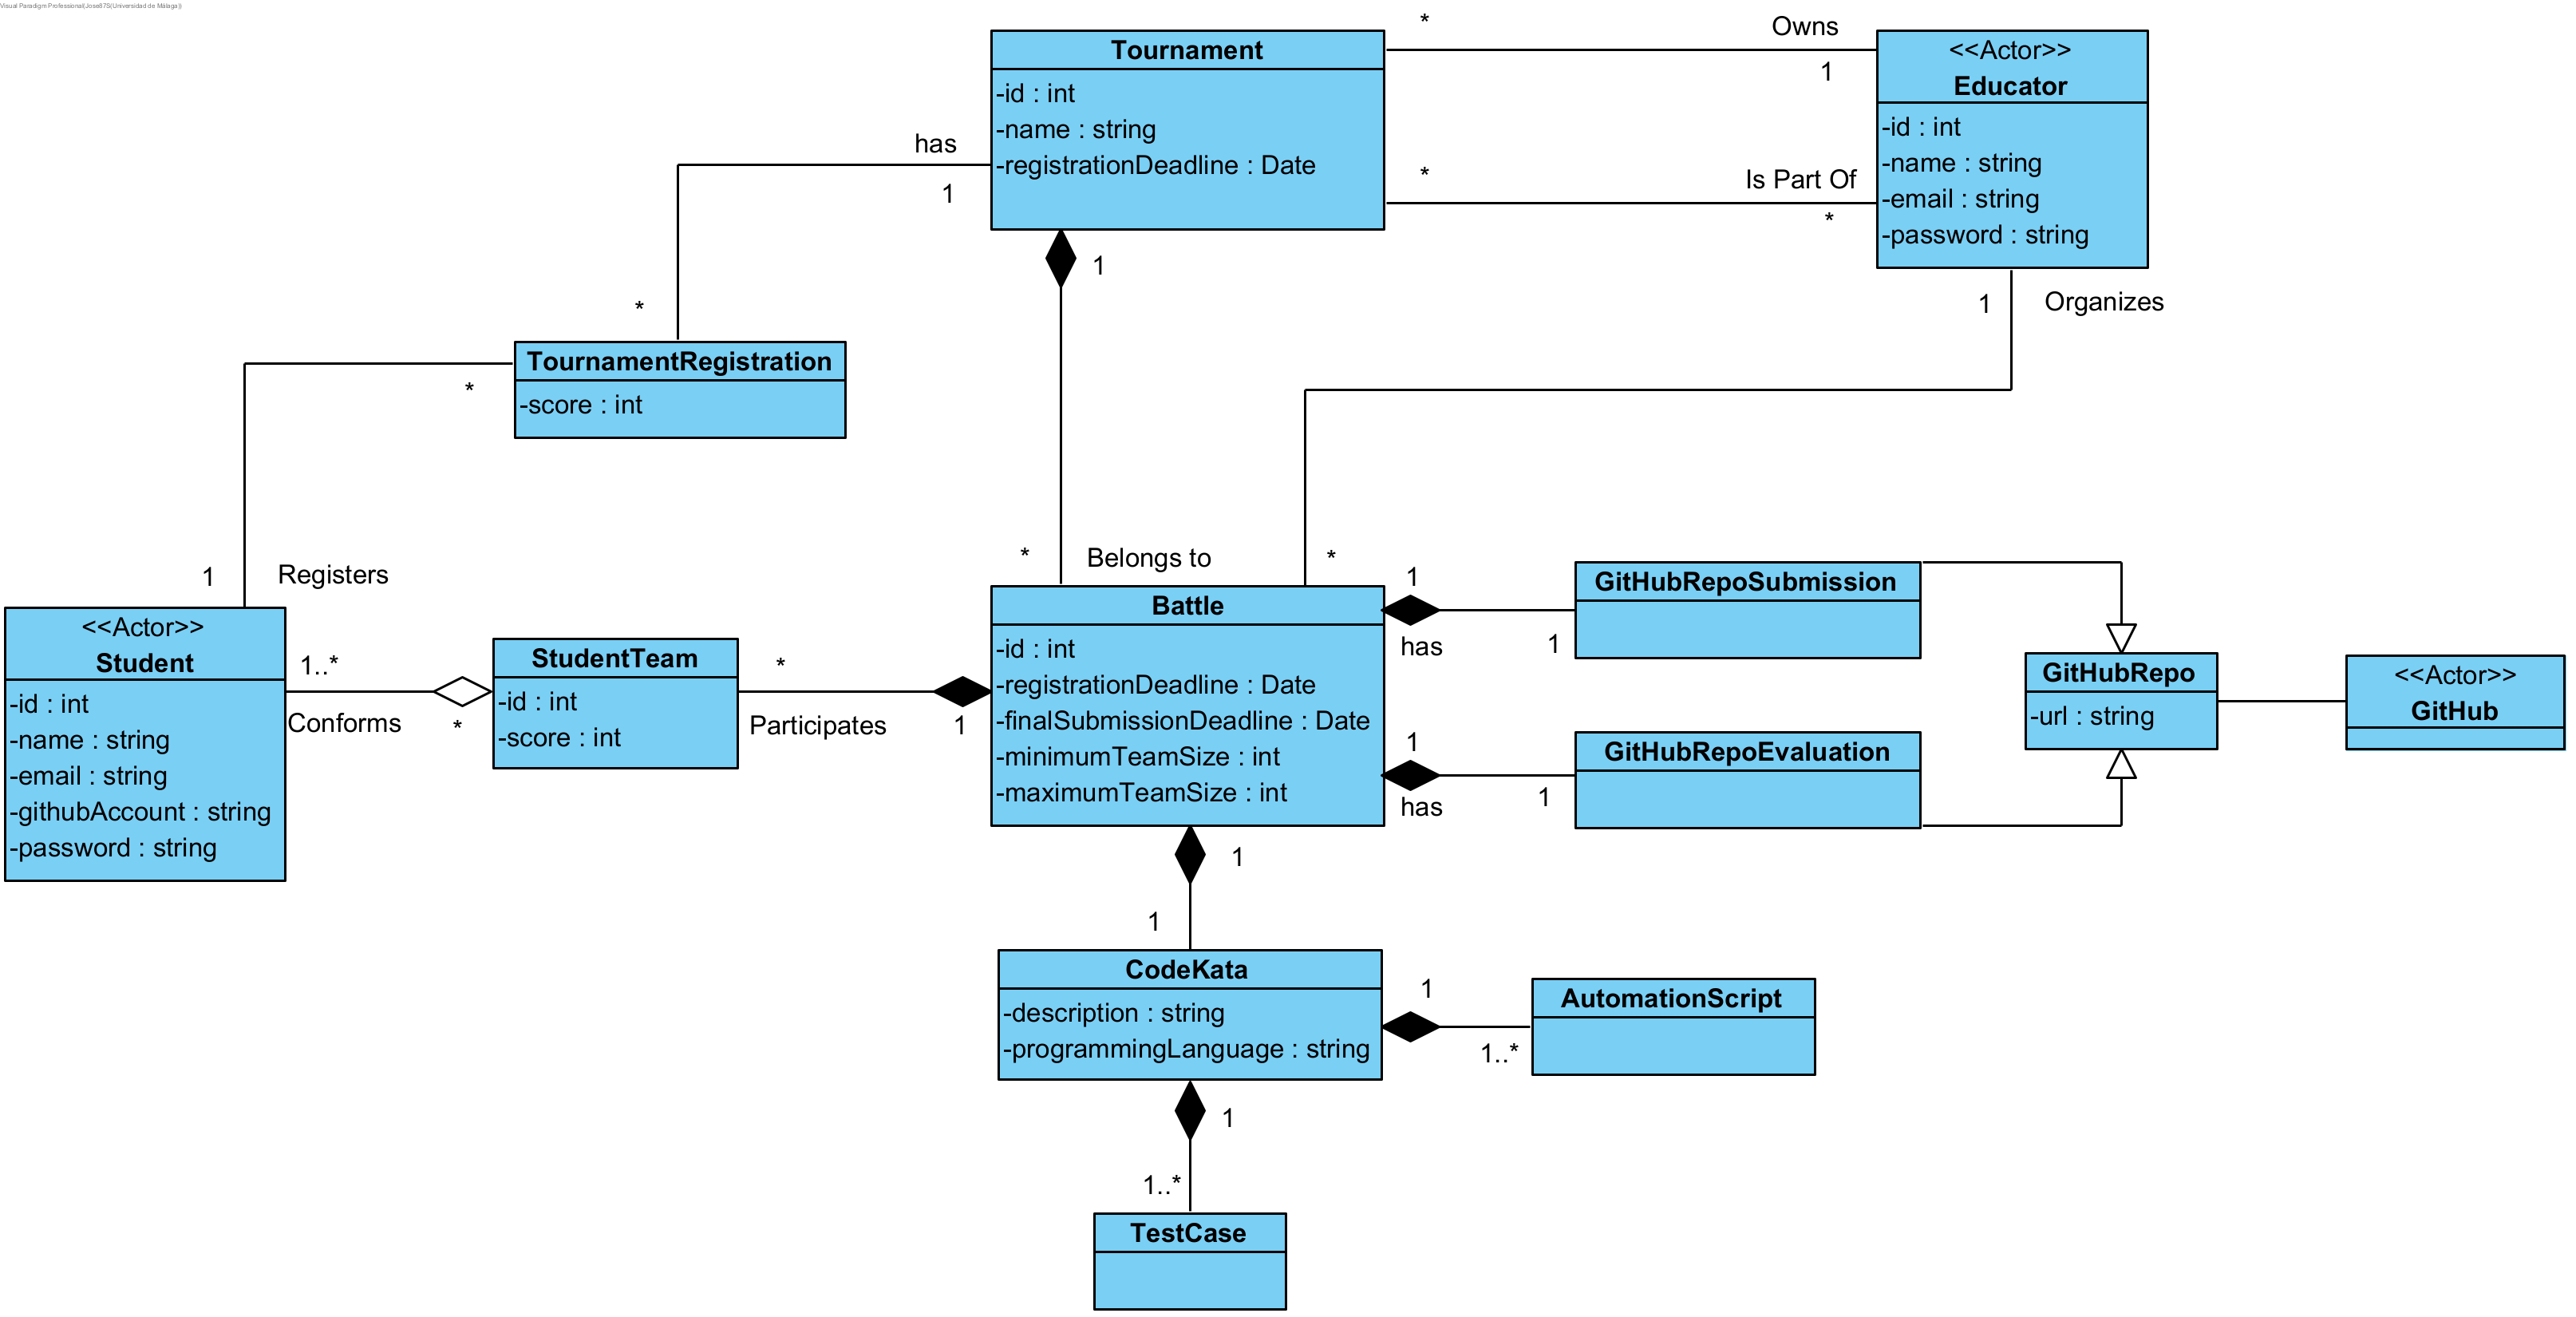
\includegraphics[width=1\textwidth]{images/DomainClassDiagram.png}
    \caption{Domain Class Diagram}
    \label{fig:DomainClassDiagram}
\end{figure}

\subsubsection{State Diagrams}

Here it is possible to see the state diagrams for the classes of the system where this is more relevant.
\begin{itemize}
    \item \textbf{Battle:}
\end{itemize}

\begin{figure}[!h]
    \centering
    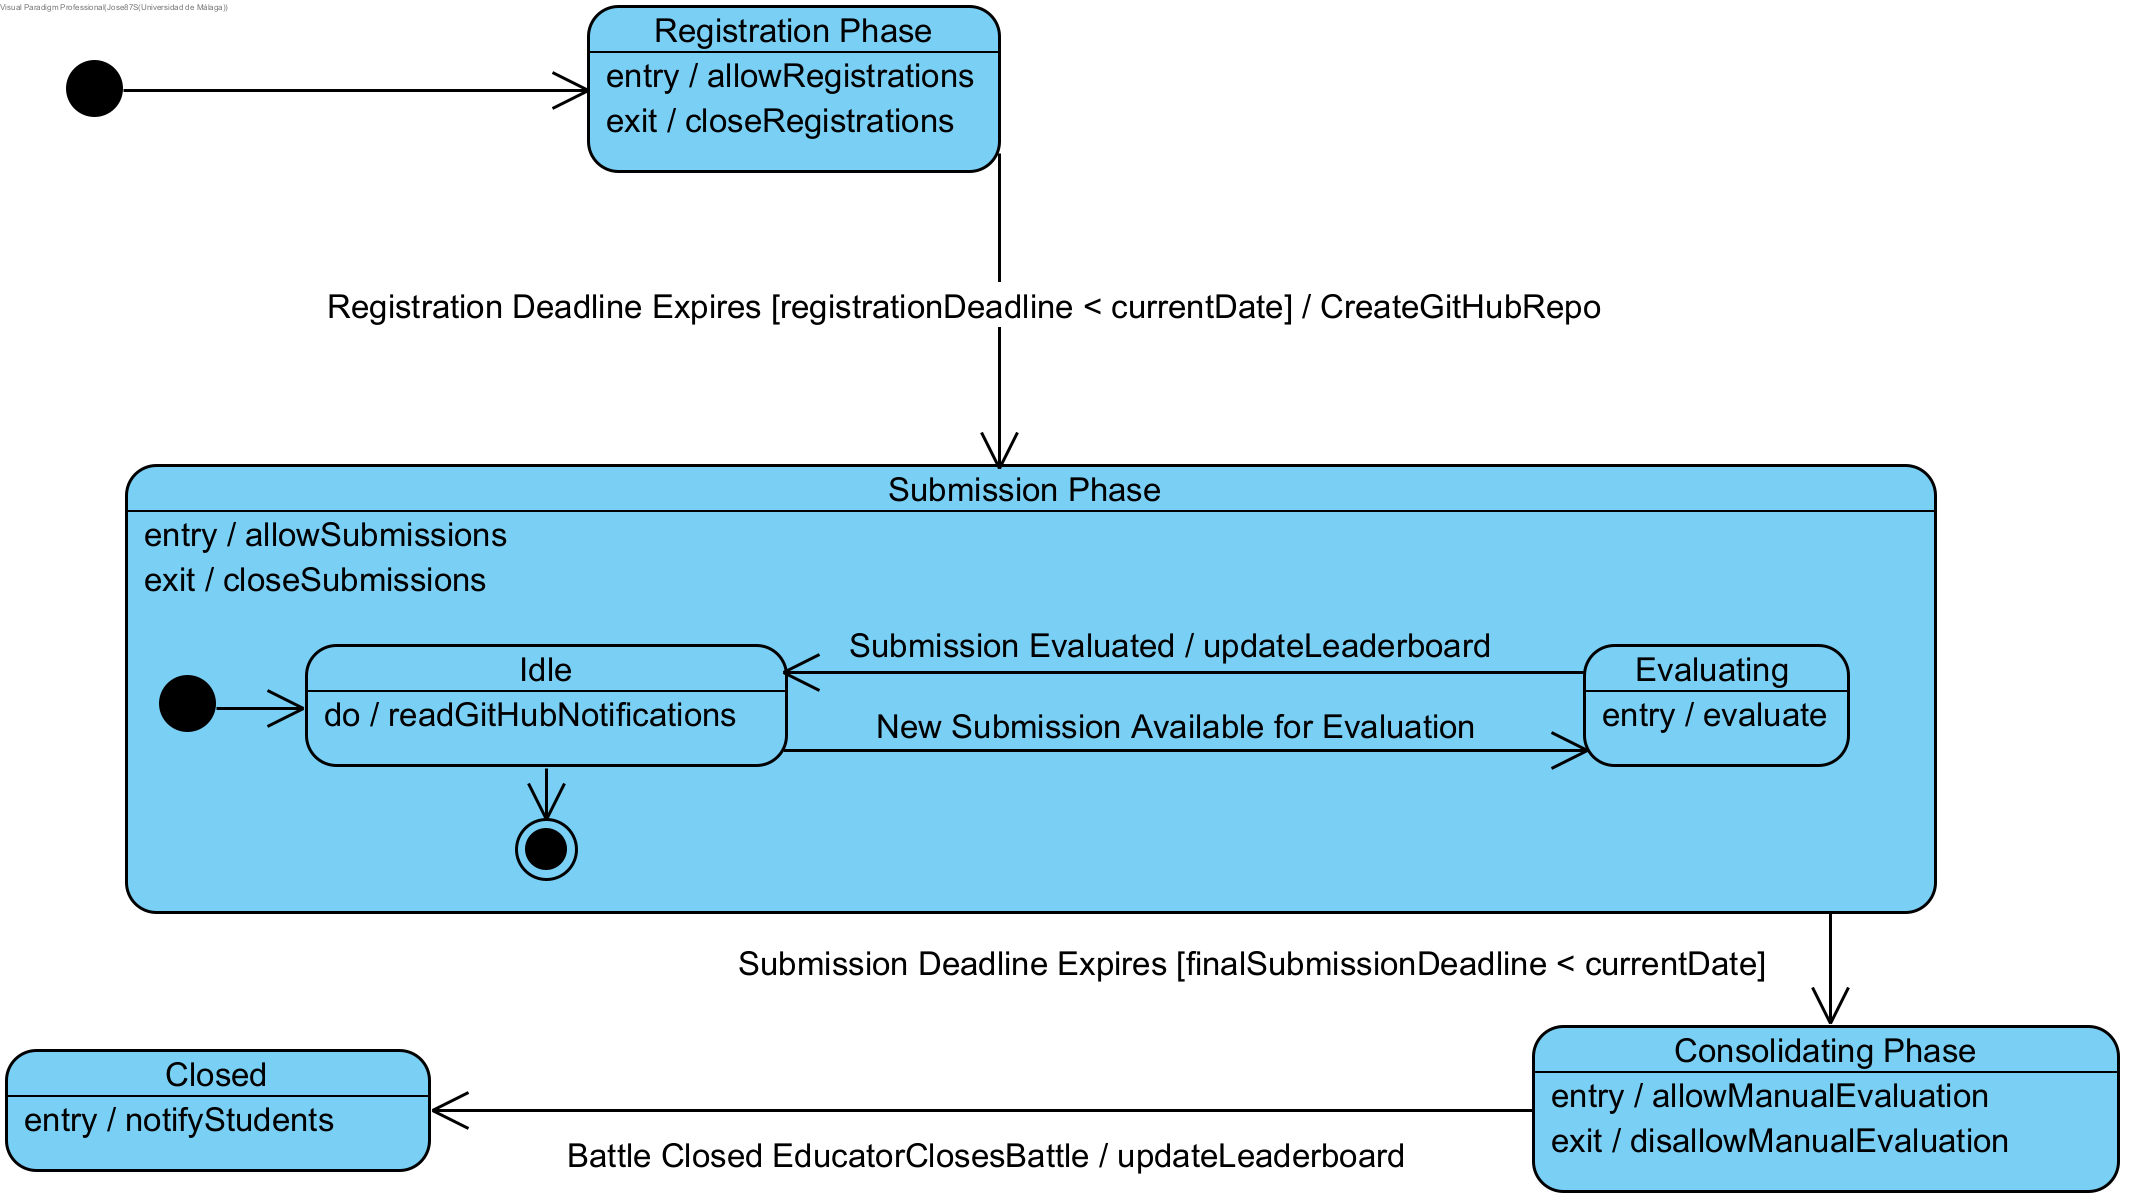
\includegraphics[width=1\textwidth]{images/BattleStateDiagram.png}
    \caption{Battle State Diagram}
    \label{fig:BattleStateDiagram}
\end{figure}

A battle is firstly on it's \textbf{Registration Phase} where StudentTeams can register to 
it. Once the registration deadline is reached, the battle moves to the 
\textbf{Submission Phase} and it creates the \textbf{GitHubRepo}. Here the \textbf{StudentTeam}s  
can submit their solutions to the battle 
through GitHub. In this state there are two substates: \textbf{Idle} and \textbf{Evaluating}. 
In the \textbf{Idle} state, the system is waiting for a notification from GitHub that a commit 
has been pushed to the main branch of one of the forked repositories of the battle. Once the system 
receives the notification, it moves to the \textbf{Evaluating} state where it runs the build 
automation scripts to evaluate the submission. Once the evaluation is done, the system updates 
the leaderboard of the battle and moves back to the \textbf{Idle} state. Once the final submission 
deadline is reached, the battle moves to the \textbf{Consolidation Phase} where the \textbf{Educator} that 
created the battle can perform manual evaluations on the submissions of the \textbf{Student}s. 
Once the \textbf{Educator} consolidates the results of the battle, the battle moves to the \textbf{Closed} 
state updating the leaderboard of the battle with the \textbf{Educator}'s evaluations. Here the system 
notifies the \textbf{Student}s that the final results have been published.

\begin{itemize}
    \item \textbf{Tournament:}
\end{itemize}

\begin{figure}[!h]
    \centering
    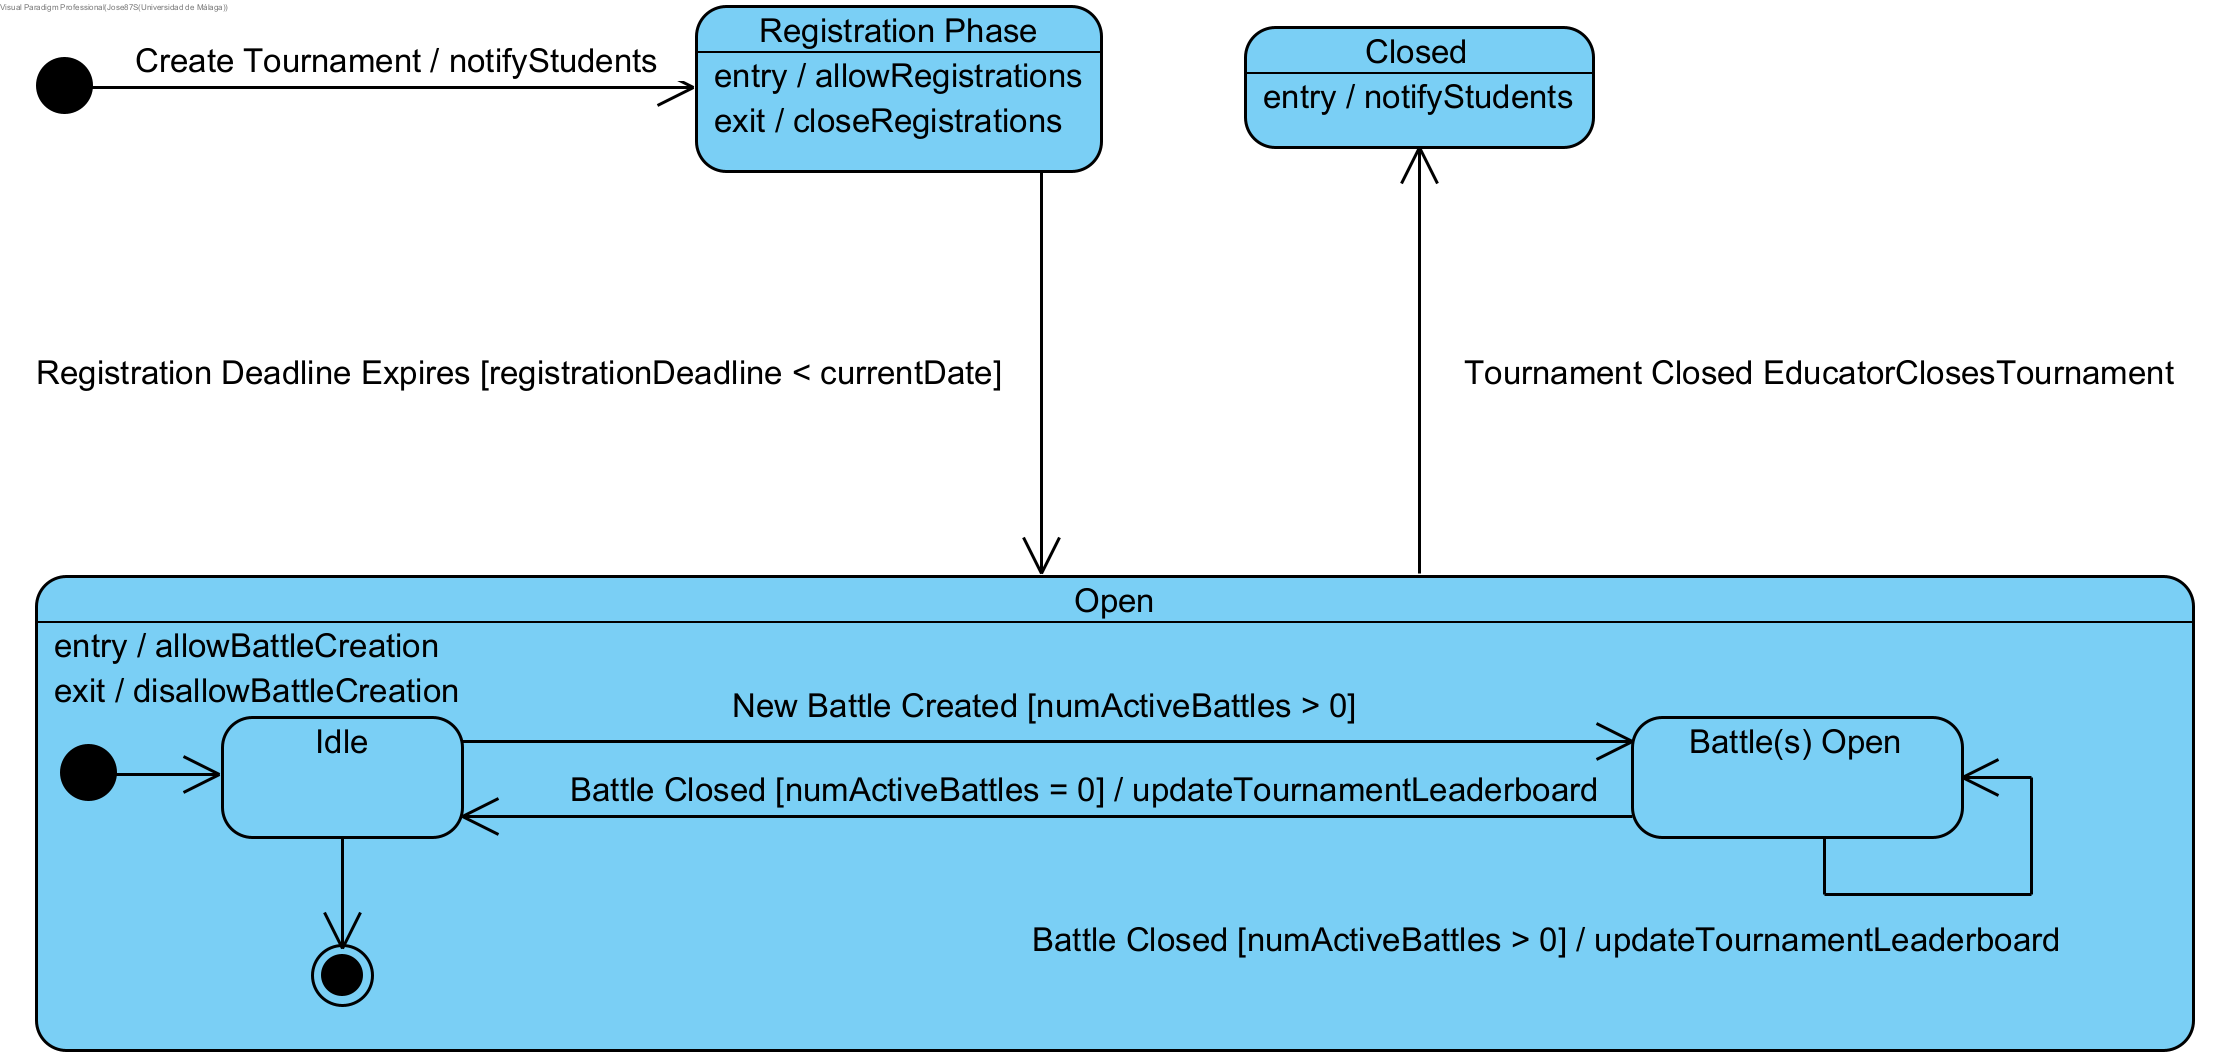
\includegraphics[width=1\textwidth]{images/TournamentStateDiagram.png}
    \caption{Tournament State Diagram}
    \label{fig:TournamentStateDiagram}
\end{figure}

When a \textbf{Tournament} is created, all students are notified. A \textbf{Tournament}, similar a \textbf{Battle}, has a \textbf{Registration Phase} where \textbf{Student}s can register to it.
Once the registration deadline is reached, the \textbf{Tournament} moves to the \textbf{Open} state. Here all the \textbf{Educator}s
that are part of the \textbf{Tournament} can create \textbf{Battle}s. The \textbf{Open} state has two substates: \textbf{Idle} 
and \textbf{Battle(s) Open}. In the \textbf{Idle} state, there are no active \textbf{Battle}s in the \textbf{Tournament}. Once an
\textbf{Educator} creates a battle, the \textbf{Tournament} moves to the \textbf{Battle(s) Open} state. Each time a battle ends,
the \textbf{Tournament} leaderboard is updated. The \textbf{Tournament} moves back to the \textbf{Idle} state once there are no active \textbf{Battle}s.
The \textbf{Tournament} can move to the closed state once the owner of the \textbf{Tournament} decides to close it and there are no active \textbf{Battle}s. 
Here, \textbf{Student}s are notified that the final results are available.

\subsection{Product functions}

\begin{itemize}
    \item \textbf{Sign up and Login:}
    
    This is a basic functionality of the system. It allows for students and educators to sign up and login to the system.
    When signing up, the user must provide a name, an email, a password and a GitHub account. The system will then send a confirmation email to the user.
    Once the user confirms their email, they can login to the system.

    \item \textbf{Create Tournament:}
    
    This functionality allows for educators to create tournaments. When creating a tournament, the educator
    must provide a registration deadline and can invite other educators to the tournament. Once the tournament
    is created, the system will notify all the students that a tournament has been created. 

    \item \textbf{Register to Tournament:}
    
    This functionality allows for students to register to tournaments. When registering to a tournament which is on 
    its registration phase. Students are able to join all the tournaments which are on this phase.

    \item \textbf{Create Battle:}
    
    This functionality allows for educators to create battles. When creating a battle, the educator
    must provide a registration deadline, a final submission deadline, a minimum and maximum number of participants per group, 
    a programming language, a description of the problem, a set of test cases and a set of build automation scripts. 
    Once the battle is created, the system will notify all the students participating in the tournament that 
    a battle has been created. The system will use the files provided by the educator to create a GitHub repository for the battle.
    
    \item \textbf{Register to Battle:}
    
    This functionality allows for students to register to battles. When registering to a battle, which is on
    its registration phase, students can invite other students or accept invitations from other students to join the battle,
    always taking into account the minimum and maximum number of participants per group set by the educator.

    \item \textbf{Evaluate submissions:}
    
    This functionality allows for the system to evaluate the submissions of the students. Each time the system receives
    a notification from GitHub that a commit has been pushed to the main branch of one of the forked repositories of the battle,
    the system will pull the latest sources from that fork, upload them to the evaluation repository of the battle, run the build automation scripts
    there and receive the results of the evaluation. The system will then update the leaderboard of the battle accordingly.

    \item \textbf{Consolidate results:}
    
    Once the final submission deadline of a battle ends, the educator that created the battle can consolidate the 
    results of the battle. This means that the educator can manually evaluate the submissions of the students and 
    set a grade for each team, which will be combined with the evaluation performed by the system. Once the educator
    finishes consolidating the results, the system will update the leaderboard of the battle and notify all the students.

    \item \textbf{Close Tournament:}
    
    Once all the battles of a tournament have ended, the owner of the tournament can close it. This means that the
    system will update the leaderboard of the tournament and notify all the students that the tournament has ended.
\end{itemize}

\subsection{User characteristics}

\begin{itemize}
    \item \textbf{Students:} They participate in battles and tournaments to improve their software development skills. They can form teams, work on the battles, and submit their solutions through GitHub.
    \item \textbf{Educators:}: They are responsible for creating and managing battles and tournaments. They set various parameters for battles, evaluate the solutions submitted by students, and provide feedback.
\end{itemize}

\newpage
\subsection{Assumptions, dependencies and constraints}

\subsubsection{Domain Assumptions}

\begin{itemize}
    \item \textbf{D1:} All users have a valid email address and can access their email to confirm their registration.
    \item \textbf{D2:} GitHub integration is reliable, and the system can communicate with GitHub to create repositories, pull code, submit files, and receive notifications and reports.
    \item \textbf{D3:} Students and educators have a basic understanding of version control systems, especially GitHub.
    \item \textbf{D4:} Educators have the necessary expertise to create meaningful and effective code kata battles, including defining appropriate test cases and build automation scripts.
    \item \textbf{D5:} Students have the required technical skills to participate in code kata battles, including forking repositories, setting up GitHub Actions, and writing code.
    \item \textbf{D6:} Users have a GitHub account.
    \item \textbf{D7:} The educator's uploaded description of the problem, programming language test cases and build automation scripts are all related to each other.
    \item \textbf{D8:} Educators have a set of evaluation criteria through which they perform their manual evaluations.
\end{itemize}

\subsubsection{Dependencies}

\begin{itemize}
    \item The system relies on GitHub for version control, code repository management, and continuous integration through GitHub Actions.
    \item Email services are required for user registration confirmation and communication.
\end{itemize}

\subsubsection{Constraints}

\begin{itemize}
    \item The system's functionality heavily depends on the reliability and availability of external services such as GitHub and to a lesser extent email services.
    \item The system's performance is constrained by the response time of GitHub services for repository creation and code evaluation.
    \item Users must have internet access to interact with the CKB platform and GitHub services.
\end{itemize}

\section{SPECIFIC REQUIREMENTS}
\subsection{External Interface Requirements}
\subsubsection{User Interfaces}

In the following figures we can see the mockups of the user interfaces of the system. 

\begin{figure}[!h]
    \centering
    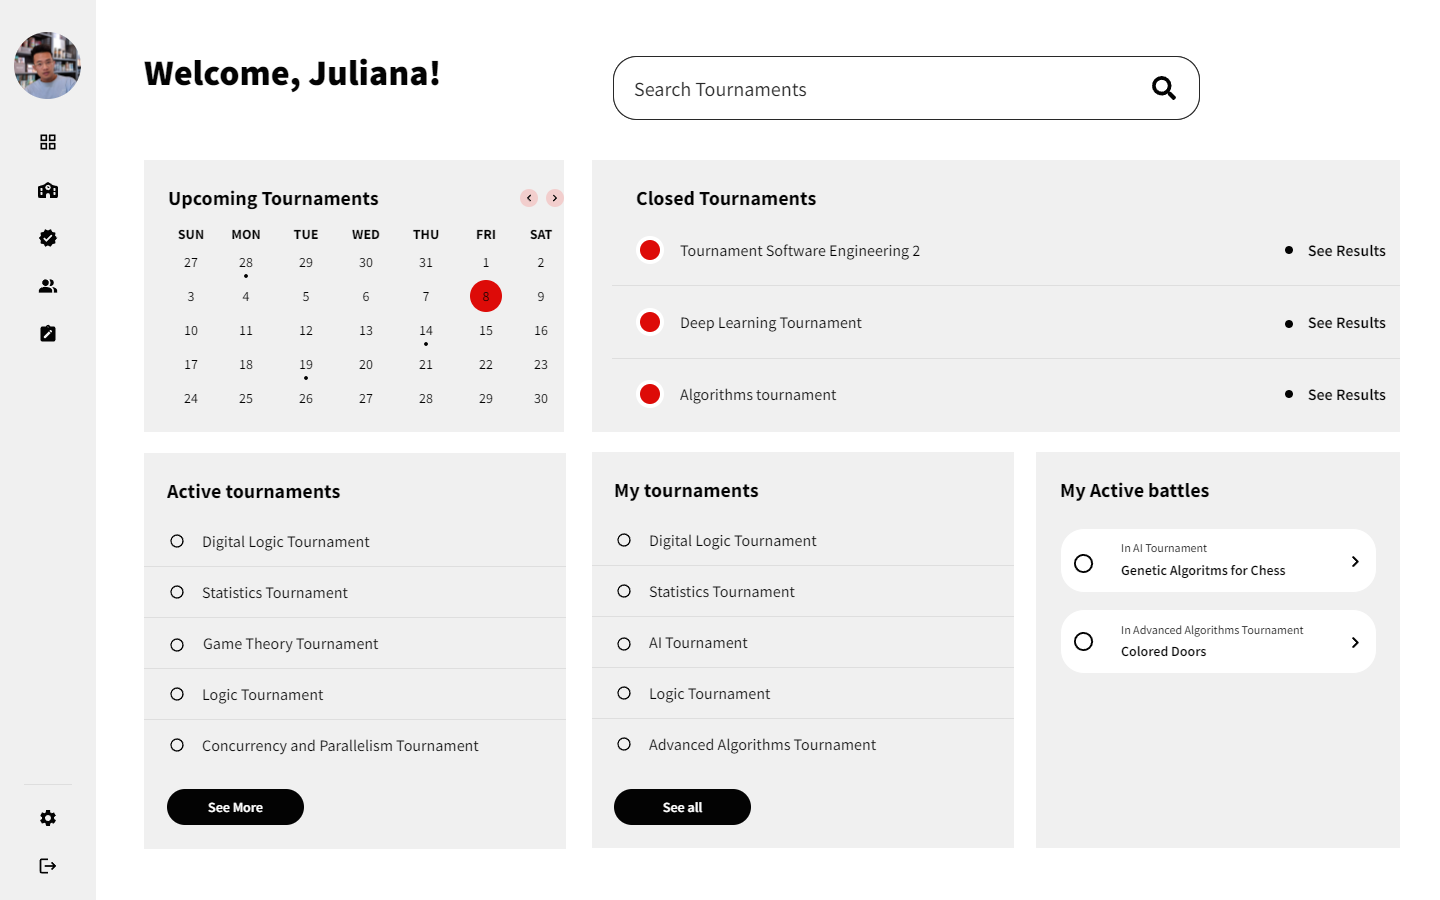
\includegraphics[width=1\textwidth]{images/UI/Homescreen Student.png}
    \caption{Homescreen Student}
    \label{fig:HomescreenStudent}
\end{figure}

The first oneis the main page of the system once a student has logged in. Here the user can see the 
list of tournaments active, another sectionwith the list of tournaments that have ended, a section 
with only the list of tournaments the student has registered to and lastly a section with the battles 
the student has registered to.

\newpage

\begin{figure}[!h]
    \centering
    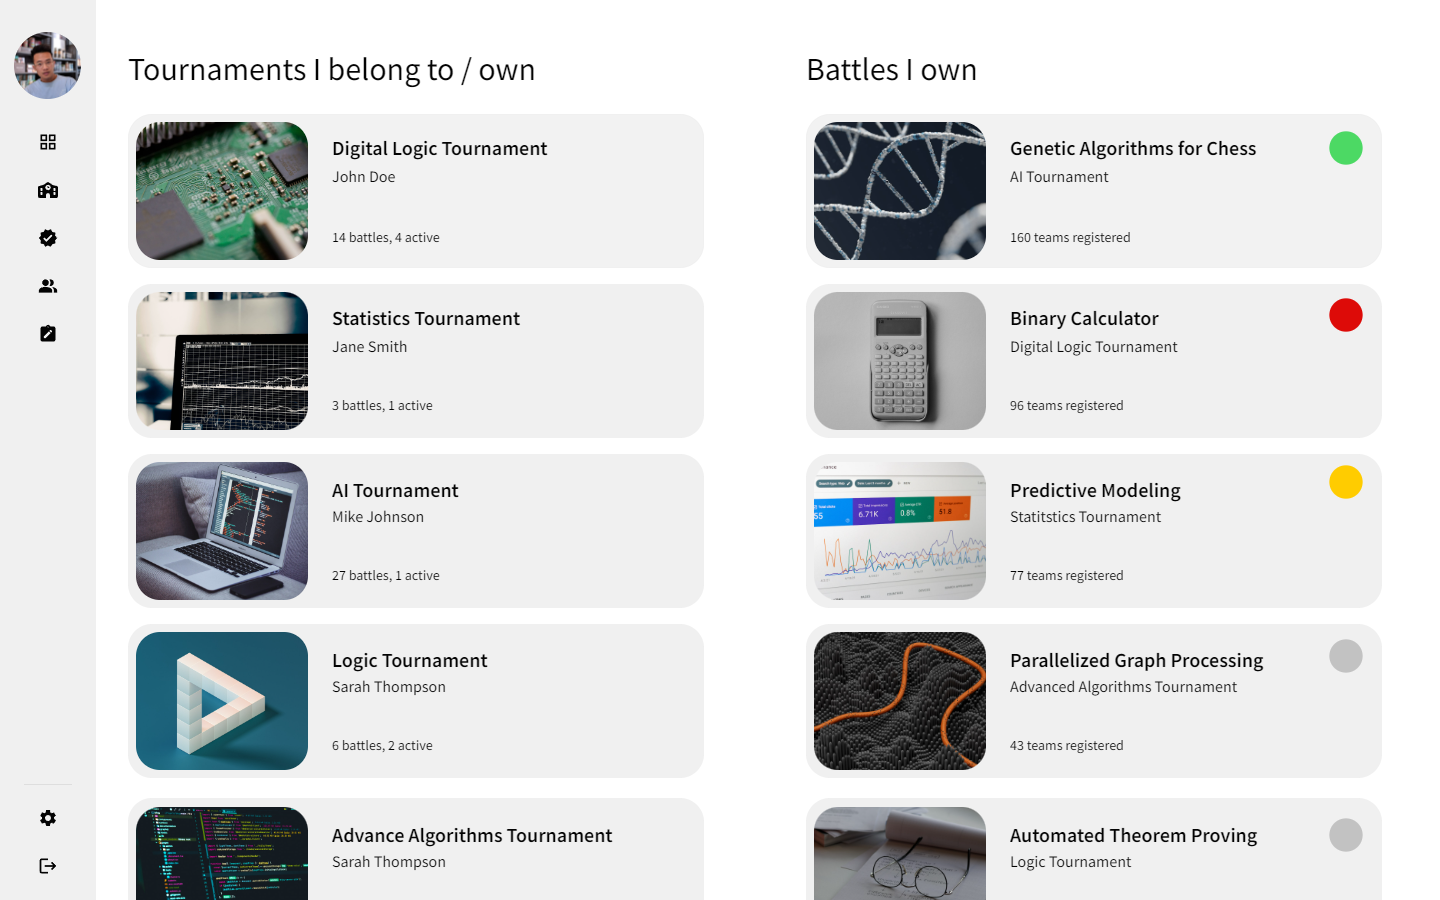
\includegraphics[width=1\textwidth]{images/UI/Educator's tournaments-battles}
    \caption{Educator's tournaments and battles}
    \label{fig:Educatorstournamentsbattles}
\end{figure}

The second one is the page where an educator can see all of the tournaments and battles they are a part of or own. 
Each tournament has some information about the name, creator, the number of battles and which of them are active.
The battles have their name, which tournament they belong to, the number of teams registered and which phase it is on
depending on the color of the circle. Gray means on the registration phase, green means on the submission phase, yellow
means on the consolidation phase and red means closed.

\newpage

\begin{figure}[!h]
    \centering
    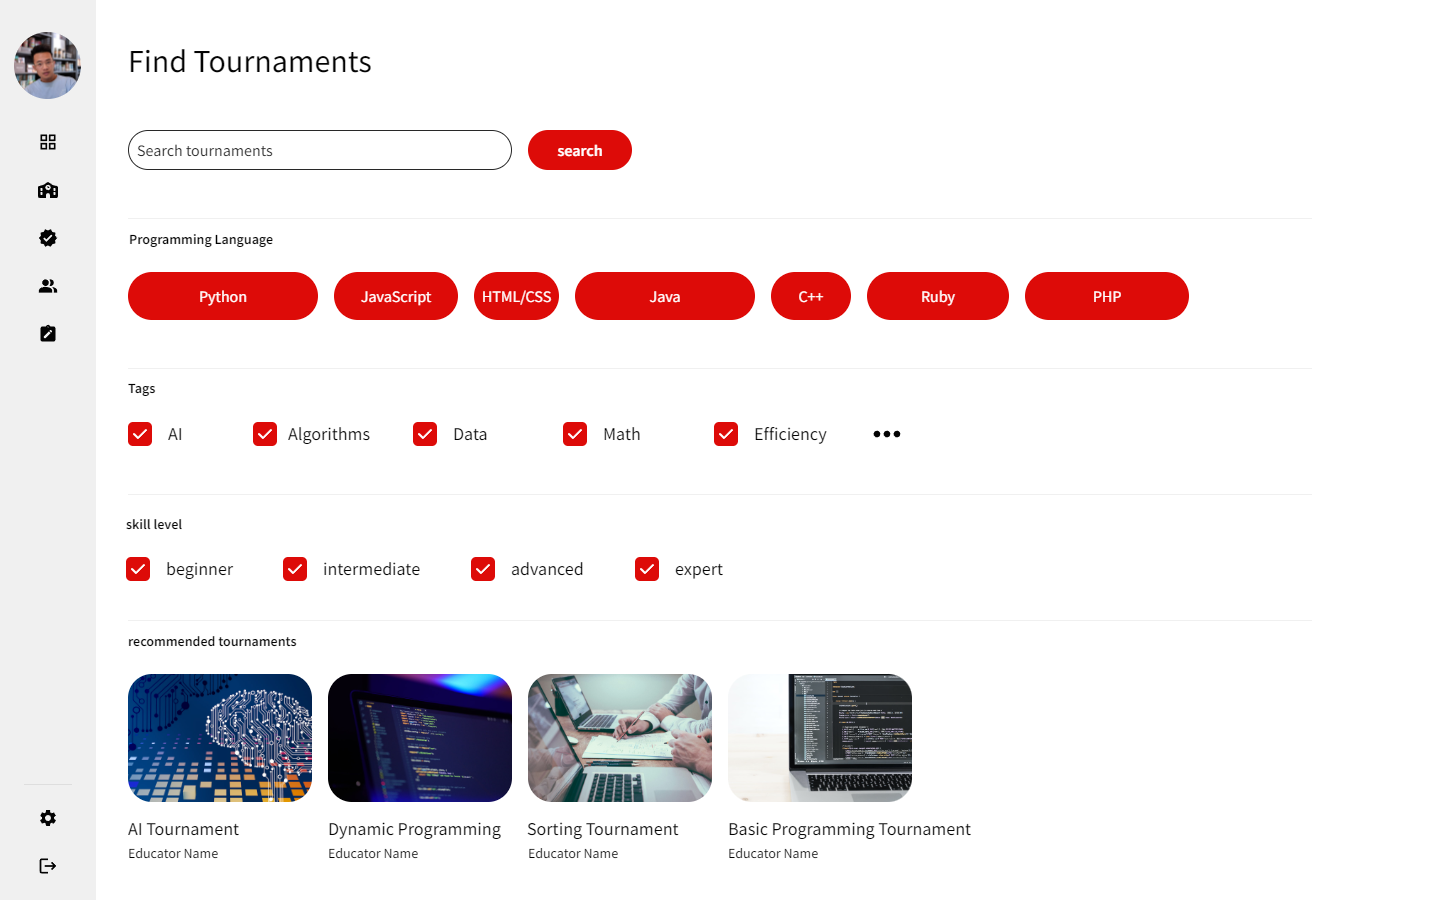
\includegraphics[width=1\textwidth]{images/UI/Search}
    \caption{Search Enviorment}
    \label{fig:Search}
\end{figure}

The third one is the page where a student can search for tournaments. They can enter key words to the
search bar and the system will return the tournaments that match the search. Also, there are some tags for
different topics, programming languages and difficulty levels that the student can use to filter the results.

\begin{figure}[!h]
    \centering
    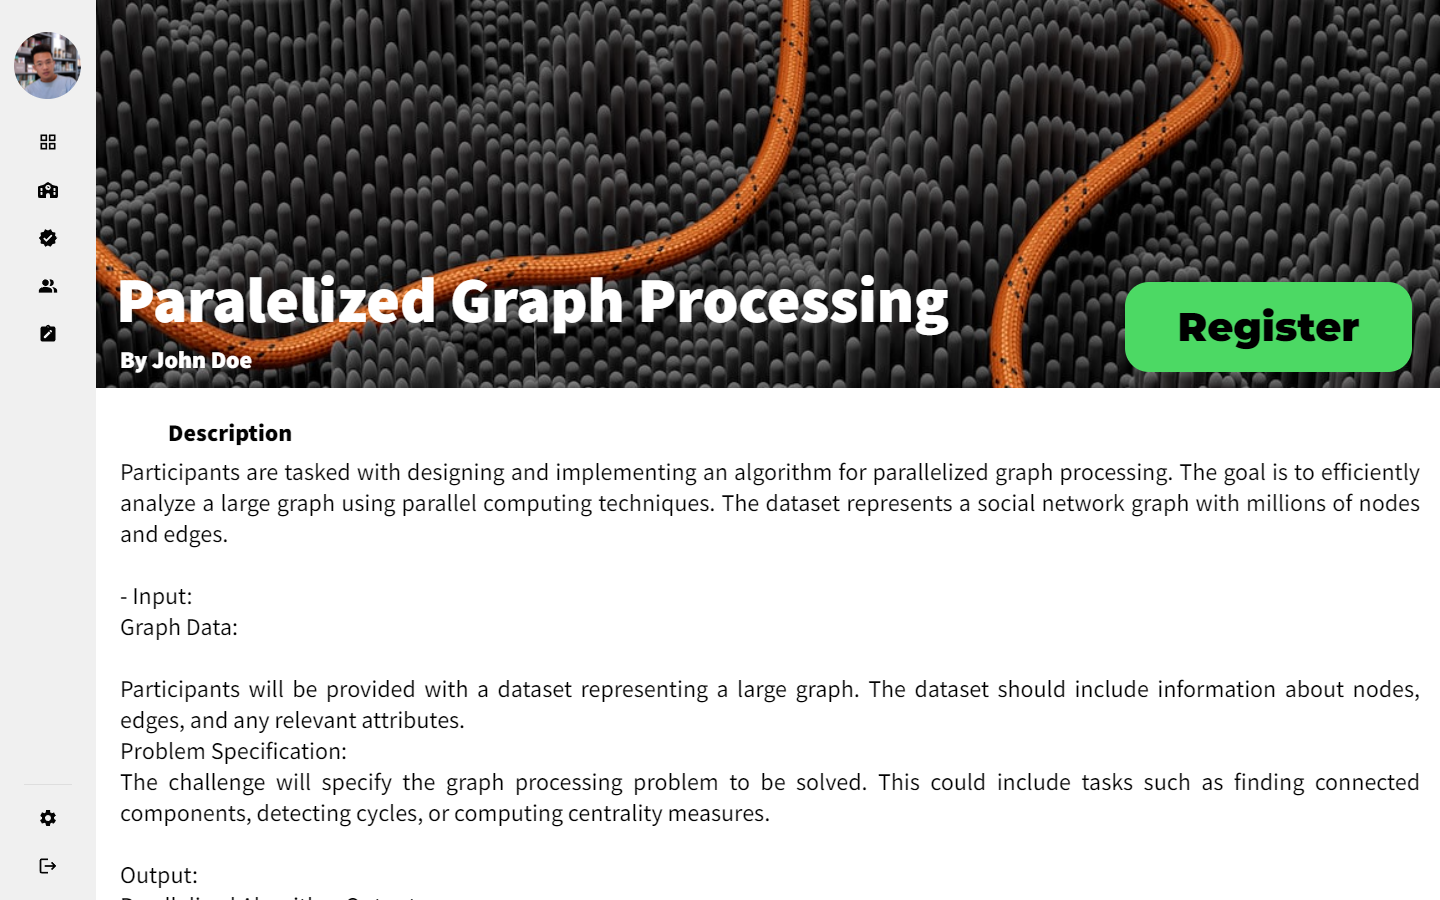
\includegraphics[width=1\textwidth]{images/UI/Battle Screen}
    \caption{Battle Screen}
    \label{fig:BattleScreen}
\end{figure}

\newpage

Lastly, the fourth one is the page where a student can see the details of a battle. Here they can see the description
of the problem, the programming language, the owner of the battle, the registration deadline and the final submission deadline.
Students can register to the battle if it is on the registration phase. When they click the button it will open a form where
they could invite other students.

\subsubsection{Hardware Interfaces}

The system will be presented in the form of an application either web or mobile or both. This means that the users
will need a device, either a computer or mobile phone to access the system. The system will also need a server to run on.

\subsubsection{Software Interfaces}

The system will interact with the following software components:

\textbf{GitHub API}: The system will communicate with the GitHub API to create repositories, receive notifications and reports, and pull and submit files.

\subsubsection{Communication Interfaces}

\textbf{Email Service}: The system relies on email services for communication purposes, including user registration confirmation and other relevant notifications.

\subsection{Functional Requirements}

\begin{itemize}
    \item \textbf{R1:} At any time, The system shall allow users to register.
    \item \textbf{R2:} At any time, The system shall allow user to login. 
    \item \textbf{R3:} At any time, The system shall allow users to try to recover their password by sending a password recovery email.
    \item \textbf{R4:} At any time, two accounts with the same email may not exist.
    \item \textbf{R5:} At any time, an account may not have a password without a number and more than 8 characters.

    \subsubsection*{Tournament and Battle Creation}

    \item \textbf{R6:} At any time, The system shall allow logged in educators to create tournaments.
    \item \textbf{R7:} When creating a tournament, the educator that is doing so must be able to set the registration deadline.
    \item \textbf{R8:} When creating a tournament, the educator that is doing so must be able to set a name.
    \item \textbf{R9:} When creating a tournament, the parameters being set must be valid. This means that the registration deadline must be in the future and the name must be a non empty string.
    \item \textbf{R10:} After the creation of a tournament, the system shall notify all the students that a tournament has been created.
    \item \textbf{R11:} At any time, The system shall allow logged in educators to invite other educators to tournaments they own and logged in educators that have been invited should be able to accept this invitations.
    \item \textbf{R12:} At any time, The system shall allow logged in educators to create battles inside tournaments they are a part of.
    \item \textbf{R13:} When creating a battle, the educator that is doing so must be able to upload a description of the problem.
    \item \textbf{R14:} When creating a battle, the educator that is doing so must be able to choose the programming language.
    \item \textbf{R15:} When creating a battle, the educator that is doing so must be able to set the registration deadline.
    \item \textbf{R16:} When creating a battle, the educator that is doing so must be able to set the final submission deadline.
    \item \textbf{R17:} When creating a battle, the educator that is doing so must be able to set the minimum and maximum number of participants per group.
    \item \textbf{R18:} When creating a battle, the educator that is doing so must be able to upload the test cases that will be used to evaluate the students' code.
    \item \textbf{R19:} When creating a battle, the educator that is doing so must be able to upload the build automation scripts that will be used to evaluate the students' code.
    \item \textbf{R20:} When creating a battle, the parameters being set must be valid. This means that the registration deadline must be in the future, the final submission deadline must be after the registration deadline, the minimum number of participants per group must be greater than 0, the maximum number of participants per group must be greater than or equal to the minimum number of participants per group, the programming language must be a valid programming language, the description of the problem must be a non empty string, the test cases must be a valid set of test cases and the build automation scripts must be a valid set of build automation scripts. This last two vary according to the programming language.
    \item \textbf{R21:} After the creation of a battle, the system shall notify all students that are registered to the tournament the battle belongs to that a battle has been created.

    \subsubsection*{Tournament and Battle Registration}

    \item \textbf{R22:} At any time, The system shall allow logged in students to register for tournaments before the registration deadline of said tournament if they are yet not registered.
    \item \textbf{R23:} At any time, The system shall allow logged in students to cancel their registration for tournaments they belong to before the registration deadline of said tournament.
    \item \textbf{R24:} At any time, The system shall allow logged in students to register for battles of a tournament they belong to before the registration deadline of said battle if they are not registered.
    \item \textbf{R25:} When registering for a battle, the student that is doing so must be able to invite other students to the battle.
    \item \textbf{R26:} At any time, The system shall allow logged in students to accept invitations to battles of a tournament they belong to before the registration deadline of said battle.
    \item \textbf{R27:} At any time, The system shall allow logged in students to cancel their registration for battles they belong to before the registration deadline of said battle.
    
    \subsubsection*{Leaderboards}

    \item \textbf{R28:} At any time, The system shall allow logged in users to see the leaderboard of any tournament.
    \item \textbf{R29:} At any time, The system shall allow logged in users to see the leaderboard of any battle.
    
    \subsubsection*{Submissions and Evaluations}

    \item \textbf{R30:} When the registration deadline of a battle expires, the system shall create a GitHub repository for the battle that the students should fork to make submissions. This repository should have the GitHub Actions workflow set up to receive notifications from GitHub when a commit is pushed to the main branch. This way, when students fork the GitHub actions of the fork will be already set up.
    \item \textbf{R31:} When the registration deadline of a battle expires, the system shall create a GitHub repository with the appropriate files, including the automation scripts and test cases files for the battle that the system will use to evaluate the submissions of the students.
    \item \textbf{R32:} When the registration deadline of a battle expires, the system shall send invitations to the GitHub repository used for submissions of the battle to the students that registered for it.
    \item \textbf{R33:} At any time, the system should be able to receive notifications from GitHub that a commit has been pushed to the main branch of one of the forked repositories of the battle.
    \item \textbf{R34:} The system should be able to pull the latest sources from the forked repository of the battle that the notification came from.
    \item \textbf{R35:} The system should be able to upload the latest sources from the forked repository of the battle that the notification came from, to the evaluation repository of the battle.
    \item \textbf{R36:} The system should be able to receive the results of the evaluation from the evaluation repository of the battle.
    \item \textbf{R37:} The system should be able to update the leaderboard of the battle with the results of the evaluation and the timeliness of the submission.
    
    \subsubsection*{Manual Evaluations}

    \item \textbf{R38:} Once the final submission deadline of a battle expires, the system shall allow the educator that created the battle to manually evaluate the submissions of the students.
    
    \subsubsection*{Battle and Tournament Closing}

    \item \textbf{R39:} Once the educator that created the battle finishes manually evaluating the submissions of the students and closes the battle, the system shall notify all the students that participated in the battle that the final results have been published.
    \item \textbf{R40:} Once the educator that created the battle finishes manually evaluating the submissions of the students and closes the battle, the system shall update the leaderboard of the tournament that the battle belongs to by adding the score that each student got on the battle to their score on the rest of the battles of the tournament that they have participated in.
    \item \textbf{R41:} At any time, if there are no open battles in a tournament, the system shall allow the owner of the tournament to close it.
    \item \textbf{R42:} Once the owner of a tournament closes it, the system shall update the leaderboard of the tournament and notify all the students that participated in it that the tournament has ended.
    
    \subsubsection*{Search system}

    \item \textbf{R43:} At any time, the system shall allow logged in users to search for tournaments. The system should return the tournaments that match the search criteria. This criteria is given by the keywords the user searched for, the tags the user selected, the programming language the user selected and the difficulty level the user selected.
    \item \textbf{R44:} At any time, the system shall display to students the tournaments they are registered to.
    \item \textbf{R45:} At any time, the system shall display to students the battles they are registered to.
    \item \textbf{R46:} At any time, the system shall display to educators the tournaments own or are a part of.
    \item \textbf{R47:} At any time, the system shall display to educators the battles they own.
    \item \textbf{R48:} At any time, the system shall display to users that are inside a tournament the battles of that tournament.


\end{itemize}
\newpage
\subsubsection{Use Case Diagram}

The following figure shows the use case diagram of the system. It includes all the subsystems and how they interact with each other and
the actors.

\begin{figure}[!h]
    \centering
    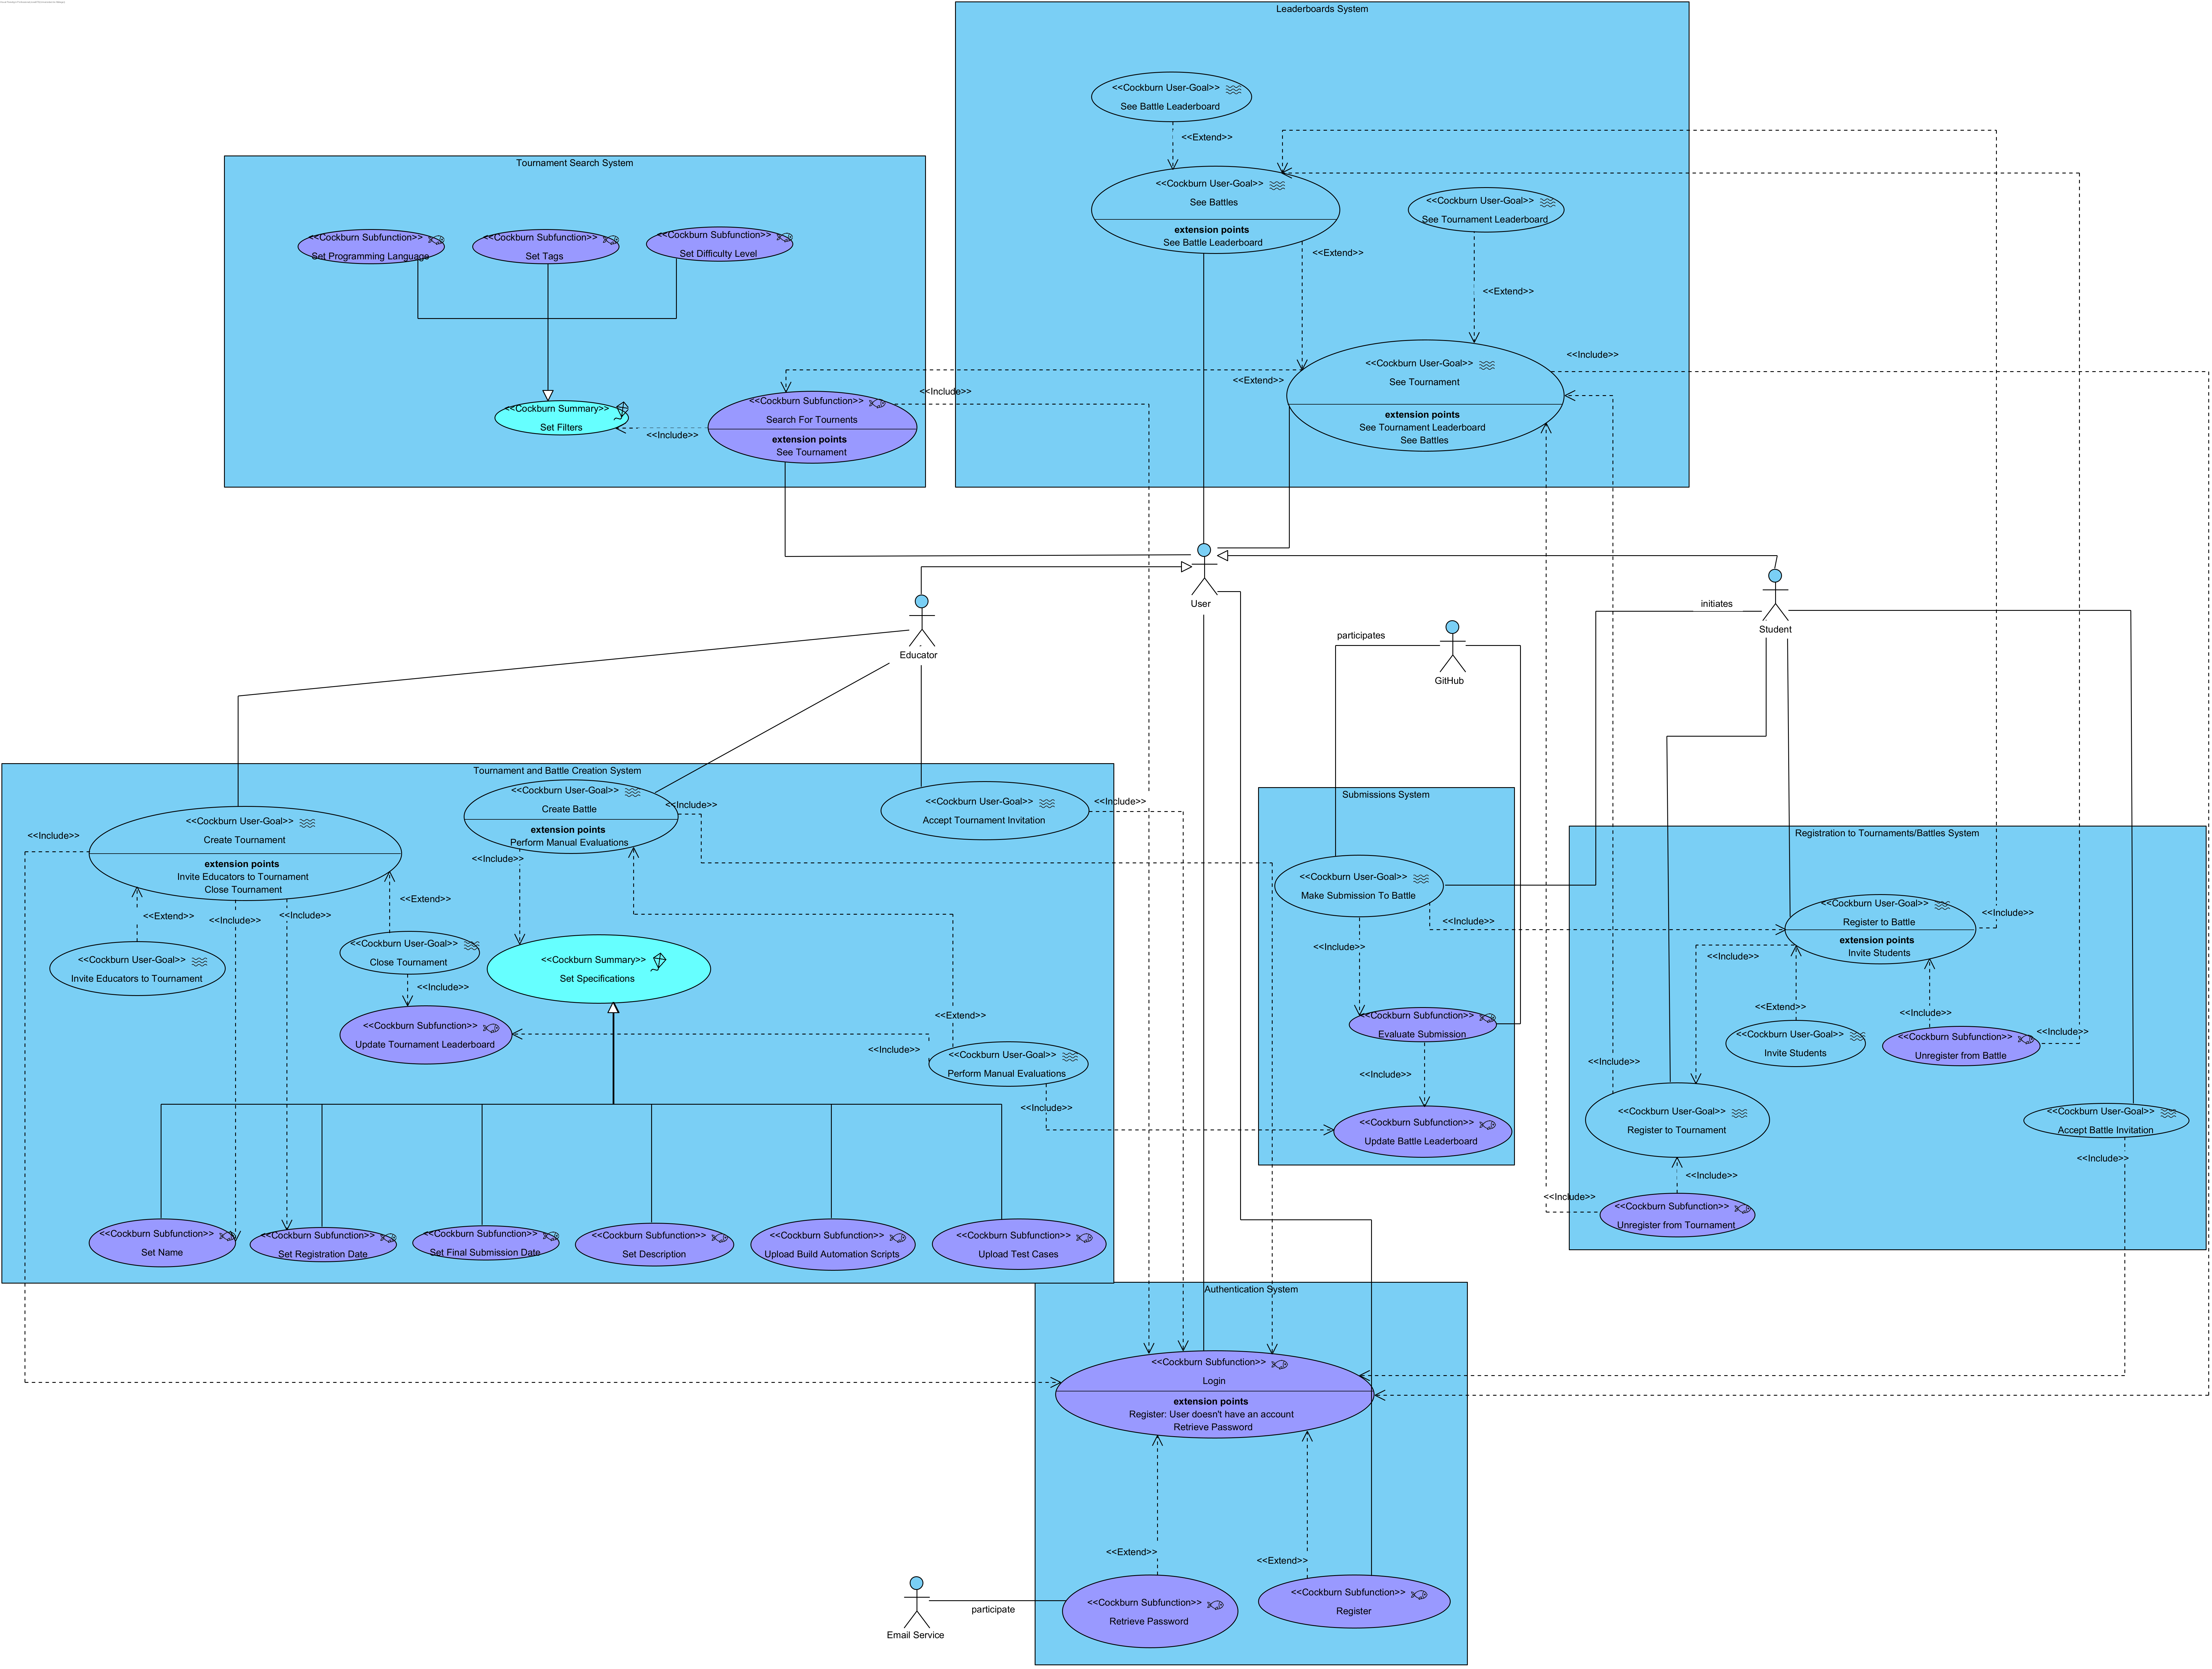
\includegraphics[width=1\textwidth]{images/UseCaseDiagram}
    \caption{Use Case Diagram}
    \label{fig:UseCaseDiagram}
\end{figure}

\subsubsection{Use Cases}

\subsubsection*{UC1 - Login}

\setlength\tabcolsep{0pt}
\begin{tabular*}{\linewidth}{@{\extracolsep{\fill}} cc }
    \hline
    Name & Login \\ 
    \hline
    Actors & user \\ 
    \hline
    Entry Condition & user is not logged in and enters the system \\ 
    \hline
    Event Flow & 1- Sytem shows registration form\\
               & 2- user enters and sends credentials\\ 
               & 3- System checks credentials\\
               & 4- Credentials are valid: System logs in user and shows initial screen\\
    \hline
    Exit Condition & user has access to all the functionalities their role allow\\ 
    \hline
    Exception & 4- Credential are not valid: System displays log in error\\ 
    \hline
\end{tabular*}

\subsubsection*{UC2 - Retrieve Password}

\setlength\tabcolsep{0pt}
\begin{tabular*}{\linewidth}{@{\extracolsep{\fill}} cc }
    \hline
    Name & Retrieve Password \\ 
    \hline
    Actors & user and email service\\ 
    \hline
    Entry Condition & user is not logged in and enters the system \\ 
    \hline
    Event Flow & 1- user selects retrieve password option\\ 
               & 2- System asks for email of account\\
               & 3- user provides email of account\\
               & 4- System sends recovery email through email service\\
               & 5- user receives recovery email through email service\\
               & 6- user sets new password\\
    \hline
    Exit Condition & user account has new password\\ 
    \hline
    Exception & 3- Email is not associated with an account: System displays log in error\\ 
    \hline
\end{tabular*}

\subsubsection*{UC3 - Register}

\begin{tabular*}{\linewidth}{@{\extracolsep{\fill}} cc }
    \hline
    Name & Login \\ 
    \hline
    Actors & user \\ 
    \hline
    Entry Condition & user logged in and enters the system \\ 
    \hline
    Event Flow & 1- System shows login form\\
               & 2- user selects register\\
               & 3- System shows registration form\\
               & 4- user enters and sends new credentials\\ 
               & 5- System checks credentials\\
               & 6- Credentials are valid: System saves the credentials\\ 
    \hline
    Exit Condition & user has access now valid credentials to log in\\ 
    \hline
    Exception & 6- Credentials are not valid:\\
              &   System shows an error message\\
    \hline
\end{tabular*}

\subsubsection*{UC4 - Educator Creates Tournament}

\begin{tabular*}{\linewidth}{@{\extracolsep{\fill}} cc }
    \hline
    Name & Tournament Creation \\ 
    \hline
    Actors & educator\\ 
    \hline
    Entry Condition & educator is logged in and enters the system \\ 
    \hline
    Event Flow & 1- educator selects create tournament option\\
               & 2- System returns a tournament form to the educator\\
               & 3- educator sets tournament parameters\\
               & 4- System checks parameters\\
               & 5- Parameters valid: System creates the tournament\\
               & 6- System notifies all students\\
               & that a tournament has been created\\
    \hline
    Exit Condition & A new tournament with the given\\
                   & parameters exists in the system\\
    \hline
    Exception & 5- Parameter not valid: System shows an error message\\
    \hline
\end{tabular*}

\subsubsection*{UC5 - Educator invites other educator to tournament}

\begin{tabular*}{\linewidth}{@{\extracolsep{\fill}} cc }
    \hline
    Name & Tournament Invitation \\ 
    \hline
    Actors & educator1 and educator2 \\ 
    \hline
    Entry Condition & educator1 and educator2 are logged in, \\
                    & educator1 owns a tournament\\
                    & and has found the tournament they own\\ 
    \hline
    Event Flow & 1- educator1 looks for educator2\\
               & 2- educator1 invites educator2 to the tournament\\
               & 3- The system send notification to educator2\\    
               & 4- educator2 receives the invitation and accepts it\\
               & 5- The system adds educator2 to the tournament\\
    \hline
    Exit Condition & educator2 is now part of the tournament\\
                   &  and could create battles inside it\\
    \hline
\end{tabular*}

\subsubsection*{UC6 - Educator creates battle}

\begin{tabular*}{\linewidth}{ cc }
    \hline
    Name & Battle Creation \\ 
    \hline
    Actors & educator\\ 
    \hline
    Entry Condition & educator is part of tournament where they are creating the battle\\  
                    & the tournament registration deadline has already passed and\\
                    & educator found the tournament they want to create the battle on\\
    \hline
    Event Flow & 1- educator signals battle creation\\
               & 2- The system returns a form to the educator\\
               & 3- educator sets battle parameters, including uploading files\\
               & 4- System checks parameters\\
               & 5- Parameters valid: System creates the battle\\
               & 6- The system notifies all students \\
               & on the tournament that a battle has been created\\

    \hline
    Exit Condition & A new battle exists inside the tournament\\
    \hline
    Exception & 5- Parameters are not valid: System shows an error message\\
    \hline
\end{tabular*}

\subsubsection*{UC7 - Tournament Registration}

\begin{tabular*}{\linewidth}{@{\extracolsep{\fill}} cc }
    \hline
    Name & Tournament Registration \\ 
    \hline
    Actors & student\\ 
    \hline
    Entry Condition & student is logged in, has not registered to tournament,\\
                    & registration deadline of tournament has not expired\\
                    & and student found tournament they want to register to\\
    \hline
    Event Flow & 1- student signals they want to register to the tournament\\
               & 2- The system registers student to tournament\\
    \hline
    Exit Condition & Student is now registered to the tournament\\
    \hline
\end{tabular*}

\subsubsection*{UC8 - Tournament Unregistration}

\begin{tabular*}{\linewidth}{@{\extracolsep{\fill}} cc }
    \hline
    Name & Tournament Unregistration \\ 
    \hline
    Actors & student\\ 
    \hline
    Entry Condition & student is logged in, is registered in the tournament, its\\
                    & registration deadline has not expired and\\
                    & student found tournament they want to unregister from\\
    \hline
    Event Flow & 1- student signals they want to unregister from tournament\\
               & 2- The system unregisters student from tournament\\
    \hline
    Exit Condition & Student is not anymore on the tournament, \\
                   & which means they can no longer register to battles inside \\
                   & it once the registration deadline expires and battles are created \\
    \hline
\end{tabular*}


\subsubsection*{UC9 - Battle Registration}

\begin{tabular*}{\linewidth}{@{\extracolsep{\fill}} cc }
    \hline
    Name & Battle Registration \\ 
    \hline
    Actors & student\\ 
    \hline
    Entry Condition & student is logged in, is registered to tournament\\
                    & in which the battle exists but has not registered\\
                    & to the battle yet, the battle's\\
                    & registration deadline has not expired and\\
                    & student found battle they want to register to\\
    \hline
    Event Flow & 1- student signals they want to join battle\\
               & 2- system registers student to battle on a new team\\
    \hline
    Exit Condition & student is now registered to the battle\\
    \hline
\end{tabular*}

\subsubsection*{UC10 - Student joins battle via invite}

\begin{tabular*}{\linewidth}{@{\extracolsep{\fill}} cc }
    \hline
    Name & Battle invitation accepted \\ 
    \hline
    Actors & student1 and student2\\ 
    \hline
    Entry Condition & student1 is registered to the battle,\\
                    & student1 and student2 are \\
                    & logged in, student2 is registered to the tournament\\
                    & in which the battle exists but is not registered\\
                    & to the battle yet. The battle's registration\\
                    & deadline has not expired and student1 has found the\\
                    & battle they want to invite student2 to\\
    \hline
    Event Flow & 1- student1 looks for student2\\
               & 2- student1 signals to invite student2 to the battle\\
               & 3- The system sends invitation to student2\\ 
               & 4- student2 receives and accepts invite\\
               & 5- The system adds student2 to student1's team\\
    \hline
    Exit Condition & student2 is now registered to the battle on the same\\
                   & team as student1\\
    \hline
\end{tabular*}

\subsubsection*{UC11 - Battle Unregistration}

\begin{tabular*}{\linewidth}{@{\extracolsep{\fill}} cc }
    \hline
    Name & Battle invitation accepted \\ 
    \hline
    Actors & student\\
    \hline
    Entry Condition & student is registered to the battle,\\
                    & student is logged in, the battle's \\
                    & registration deadline has not expired\\
    \hline
    Event Flow & 1- student signals to unregister from battle\\
               & 2- The system deletes student from battle\\
    \hline
    Exit Condition & student is no longer registered to the battle\\
    \hline
\end{tabular*}

\subsubsection*{UC12 - Students makes submission}

\begin{tabular*}{\linewidth}{@{\extracolsep{\fill}} cc }
    \hline
    Name & Student makes submission \\ 
    \hline
    Actors & student and GitHub\\ 
    \hline
    Entry Condition & student is registered to a battle,\\
                    & the battle's registration deadline expired,\\
                    & the battle's final submission deadline has not expired\\
                    & and students created a fork from the repository \\
                    & the system created.\\
    \hline
    Event Flow & 1- student pushes code to the main branch\\
               & of one of the forked repositories of the battle\\
               & to GitHub.\\
               & 2- GitHub notfies the system and sends the code uploaded\\
               & 3- System pushes the code on the GitHub evaluation repository\\
               & 4- This triggers an automated workflow oN GitHub where the evaluation\\
               & is performed.\\
               & 5- The GitHub evaluation repository sends the results of the evaluation\\
               & to the system.\\
               & 6- The system updates the leaderboard of the battle with the results.\\
               & the team on the battle of the student sees the updated leaderboard.\\
    \hline.
    Exit Condition & The leaderboard of the battle has now taken into account\\
                   & the submission of the team.\\
    \hline
\end{tabular*}

\subsubsection*{UC13 - Educator Performs Manual Evaluations}

\begin{tabular*}{\linewidth}{@{\extracolsep{\fill}} cc }
    \hline
    Name & Educator performs manual evaluations and closes battle\\ 
    \hline
    Actors & educator and GitHub\\ 
    \hline
    Entry Condition & the battle's final submission deadline has expired,\\
                    & educator that owns the battle is logged in, \\
                    & the battle has not been closed and\\
                    & the educator has found the battle thet is closing\\
    \hline
    Event Flow & 1- educator asks system to see the submissions\\
               & 2- The system fetches the submissions from the GitHub evaluation repository\\
               & of the battle\\
               & 3- The system replies to the educator with the submission with more \\
               & grade of every team\\
               & 4- The educator looks at each submission and assigns a grade to it\\
               & 5- Every time the educator assigns a grade to a submission, the system\\
               & updates the leaderboard of the battle\\
               & 6- The educator finishes and notifies the system\\
               & 7- The system closes the battle, and notifies students and the \\
               & 8- The tournament it belongs to updates its leaderboard \\
               & with the results of the battle \\
    \hline.
    Exit Condition & The battle is now closed, the battle leaderboard is updated\\
                   & and the tournament leaderboard is updated\\
    \hline
\end{tabular*}

\subsubsection*{UC14 - Educator Closes Tournament}

\begin{tabular*}{\linewidth}{@{\extracolsep{\fill}} cc }
    \hline
    Name & Educator closes tournament\\ 
    \hline
    Actors & educator\\ 
    \hline
    Entry Condition & The tournament registration deadline has expired,\\
                    & the educator that owns the tournament is logged in,\\
                    & there are no open battles in the tournament that\\
                    & is being closed and educator has found the tournament\\
                    & that is closing\\
    \hline
    Event Flow & 1- educator signals system to close tournament\\
               & 2- The system closes the tournament\\
               & 3- The system updates the leaderboard of the tournament\\
               & 4- The system notifies all students that the tournament has ended\\
    \hline.
    Exit Condition  & The tournament is now closed which means that\\
                    & battles can no longer be created inside it\\
                
    \hline
    Exception & 2- There are battles still ongoing: Nothing happens\\
    \hline
\end{tabular*}

\subsubsection*{UC15 - Find Tournament via search}

\begin{tabular*}{\linewidth}{@{\extracolsep{\fill}} cc }
    \hline
    Name & User finds tournament via search\\ 
    \hline
    Actors & user\\ 
    \hline
    Entry Condition & user is logged in\\
    \hline
    Event Flow & 1- user goes to search page\\
               & 2- user enters keywords, selects tags, \\
               & selects programming language\\
               & and selects difficulty level\\
               & 3- The system returns the tournaments \\
               & that match the search criteria\\
               & 4- user selects a tournament\\
    \hline
    Exit Condition & The user is now on the tournament page\\ 
    \hline
\end{tabular*}


\subsubsection*{UC16 - Find Tournament on main page}

\begin{tabular*}{\linewidth}{@{\extracolsep{\fill}} cc }
    \hline
    Name & User finds tournament via main page\\ 
    \hline
    Actors & user\\ 
    \hline
    Entry Condition & user is logged in and\\
                    & (user is student and is registered to tournament or\\ 
                    & user is educator and is part of tournament)\\
    \hline
    Event Flow & 1- System displays tournaments on main page\\
               & 2- user selects a tournament\\
    \hline.
    Exit Condition & The user is now on the tournament page\\
                
    \hline
\end{tabular*}

\subsubsection*{UC17 - Find Battle on main page}

\begin{tabular*}{\linewidth}{@{\extracolsep{\fill}} cc }
    \hline
    Name & User finds battle via main page\\ 
    \hline
    Actors & user\\ 
    \hline
    Entry Condition & user is logged in and\\
                    & (user is student and is registered to battle or\\ 
                    & user is educator and owns battle)\\
    \hline
    Event Flow & 1- System displays battles on main page\\
               & 2- user selects a battle\\
    \hline.
    Exit Condition & The user is now on the battle page\\
                
    \hline
\end{tabular*}

\subsubsection*{UC18 - Find Battle on tournament page}

\begin{tabular*}{\linewidth}{@{\extracolsep{\fill}} cc }
    \hline
    Name & User finds battle via tournament page\\ 
    \hline
    Actors & user\\ 
    \hline
    Entry Condition & user is logged in and\\
                    & user found tournament that has battle\\
    \hline
    Event Flow & 1- System displays battles on the tournament page\\
               & 2- user selects a battle\\
    \hline.
    Exit Condition & The user is now on the battle page\\
                
    \hline
\end{tabular*}

\subsubsection{Sequence Diagrams}

On the following figures we can see the sequence diagrams of the main use cases of the system that were described above.
It is important to note that the sequence diagrams only show that particular use case, but normally
these are part of a bigger flow of events that are not shown here but can be reconstructed from the entry conditions
of the use cases. For example, the use case regarding the submission on a battle is part of the flow of events
that starts with an educator registering in the system, logging in, creating a tournament, a student registering to the tournament
the registration deadline expiring, the creation of a battle the student registering to the battle and finally the registration deadline
expiring. This dependencies are both shown on the entry conditions of the use cases and on the use case diagram.

\begin{figure}[H]
    \centering
    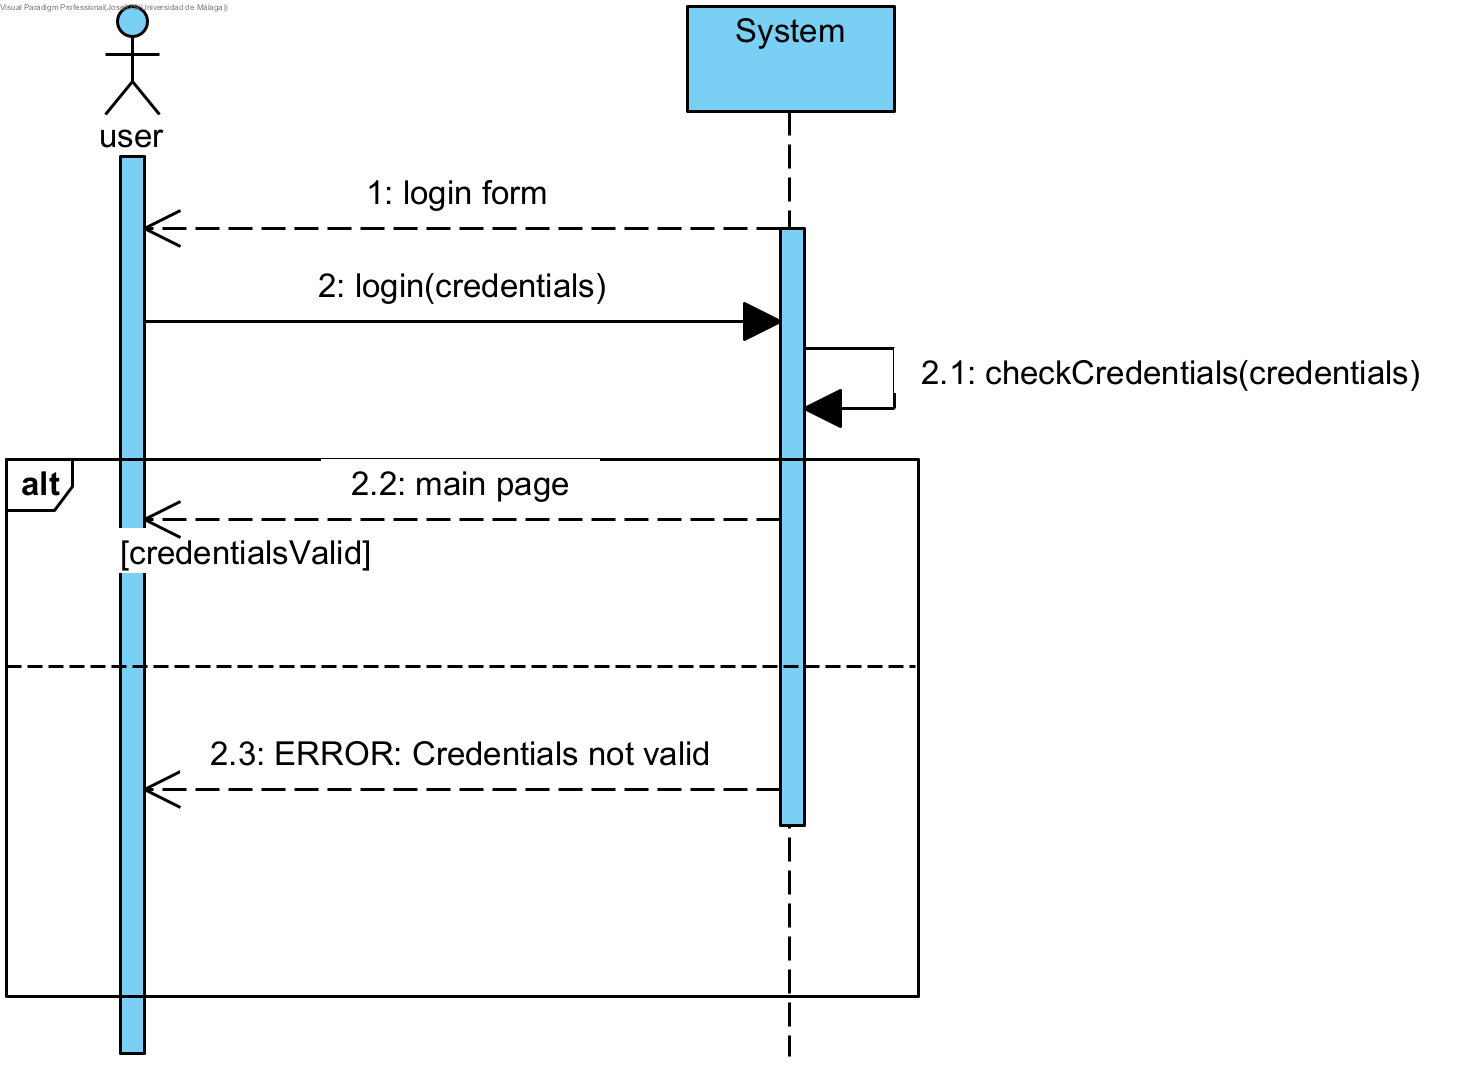
\includegraphics[width=1\textwidth]{images/UseCaseSequenceDiagrams/UC1}
    \caption{Use Case 1}
    \label{fig:UC1}
\end{figure}

\begin{figure}[H]
    \centering
    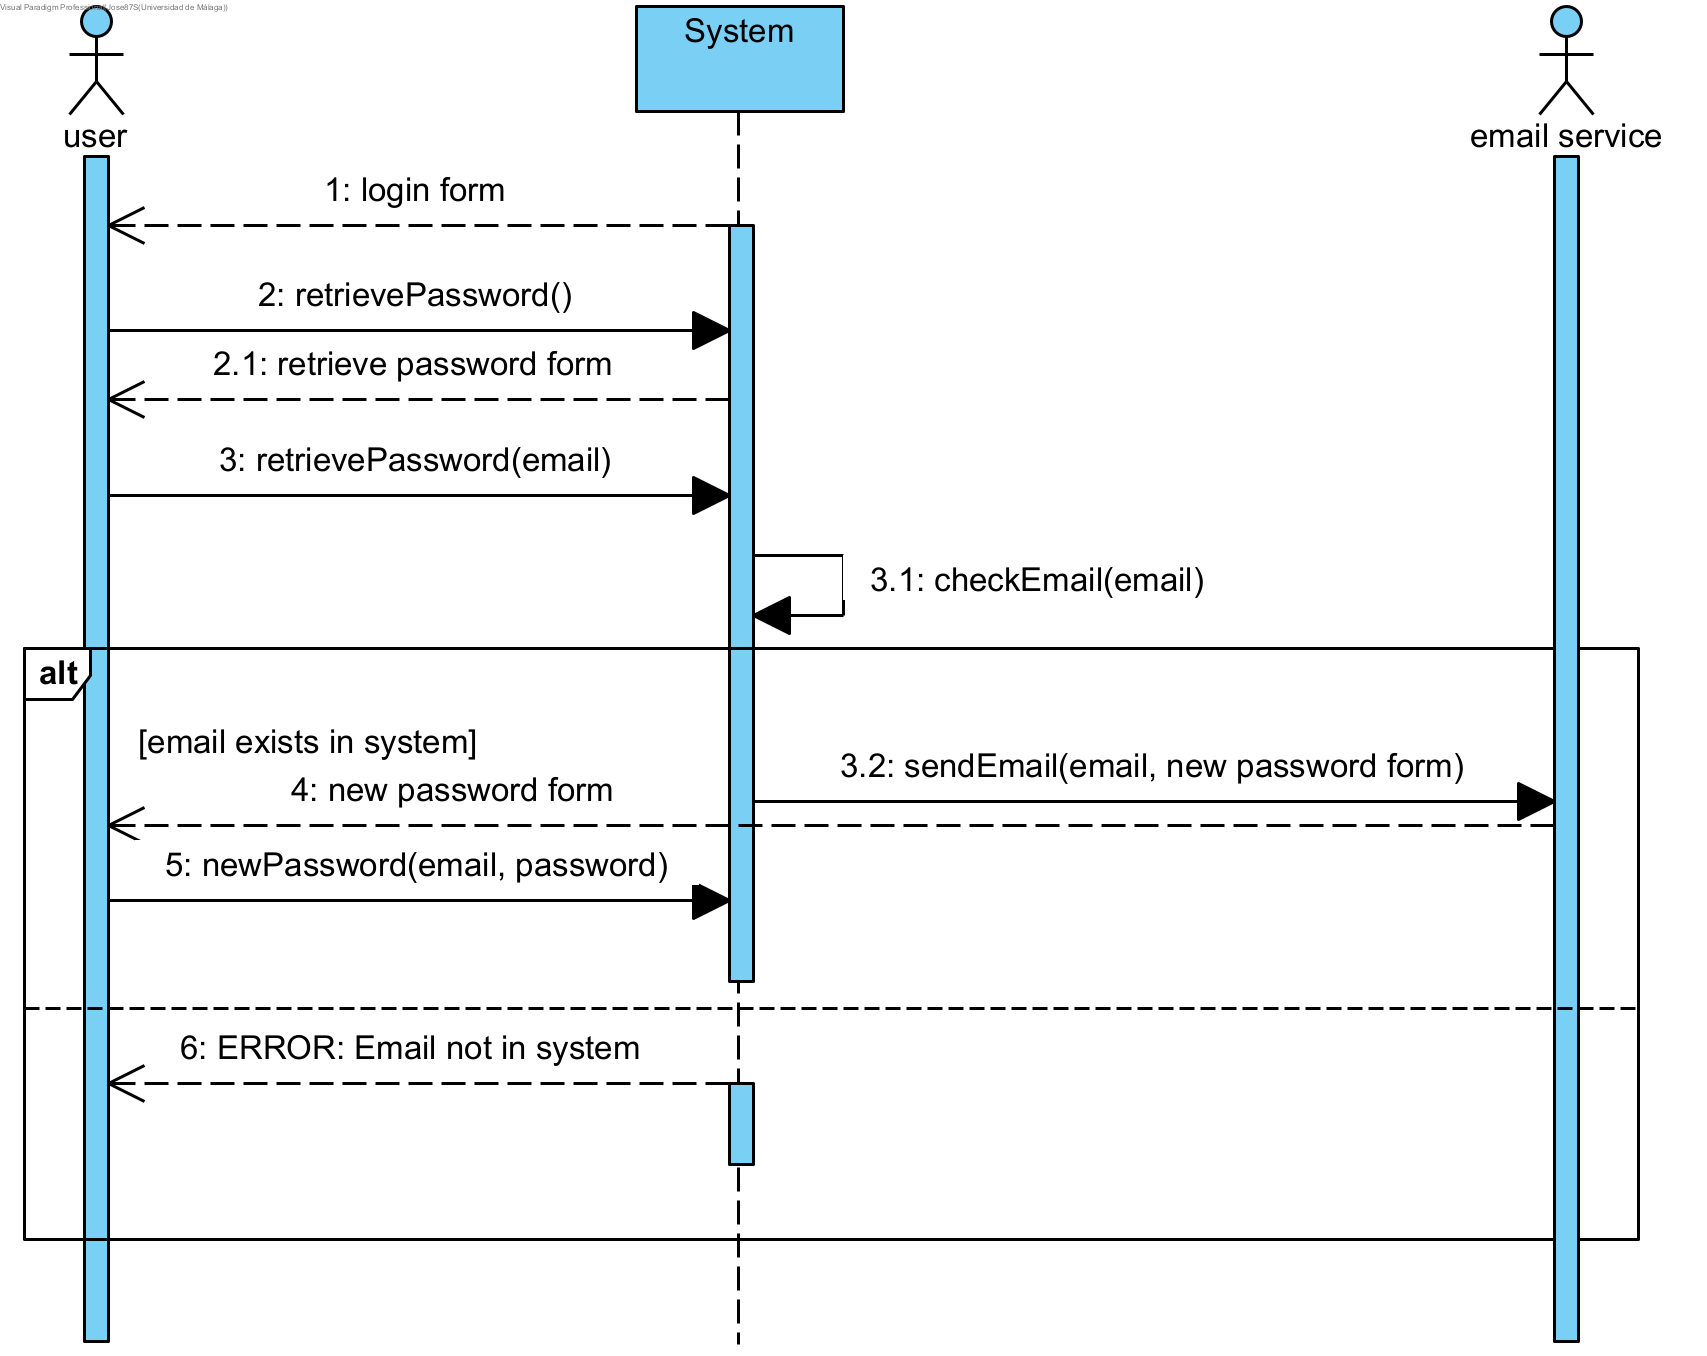
\includegraphics[width=1\textwidth]{images/UseCaseSequenceDiagrams/UC2}
    \caption{Use Case 2}
    \label{fig:UC2}
\end{figure}

\begin{figure}[H]
    \centering
    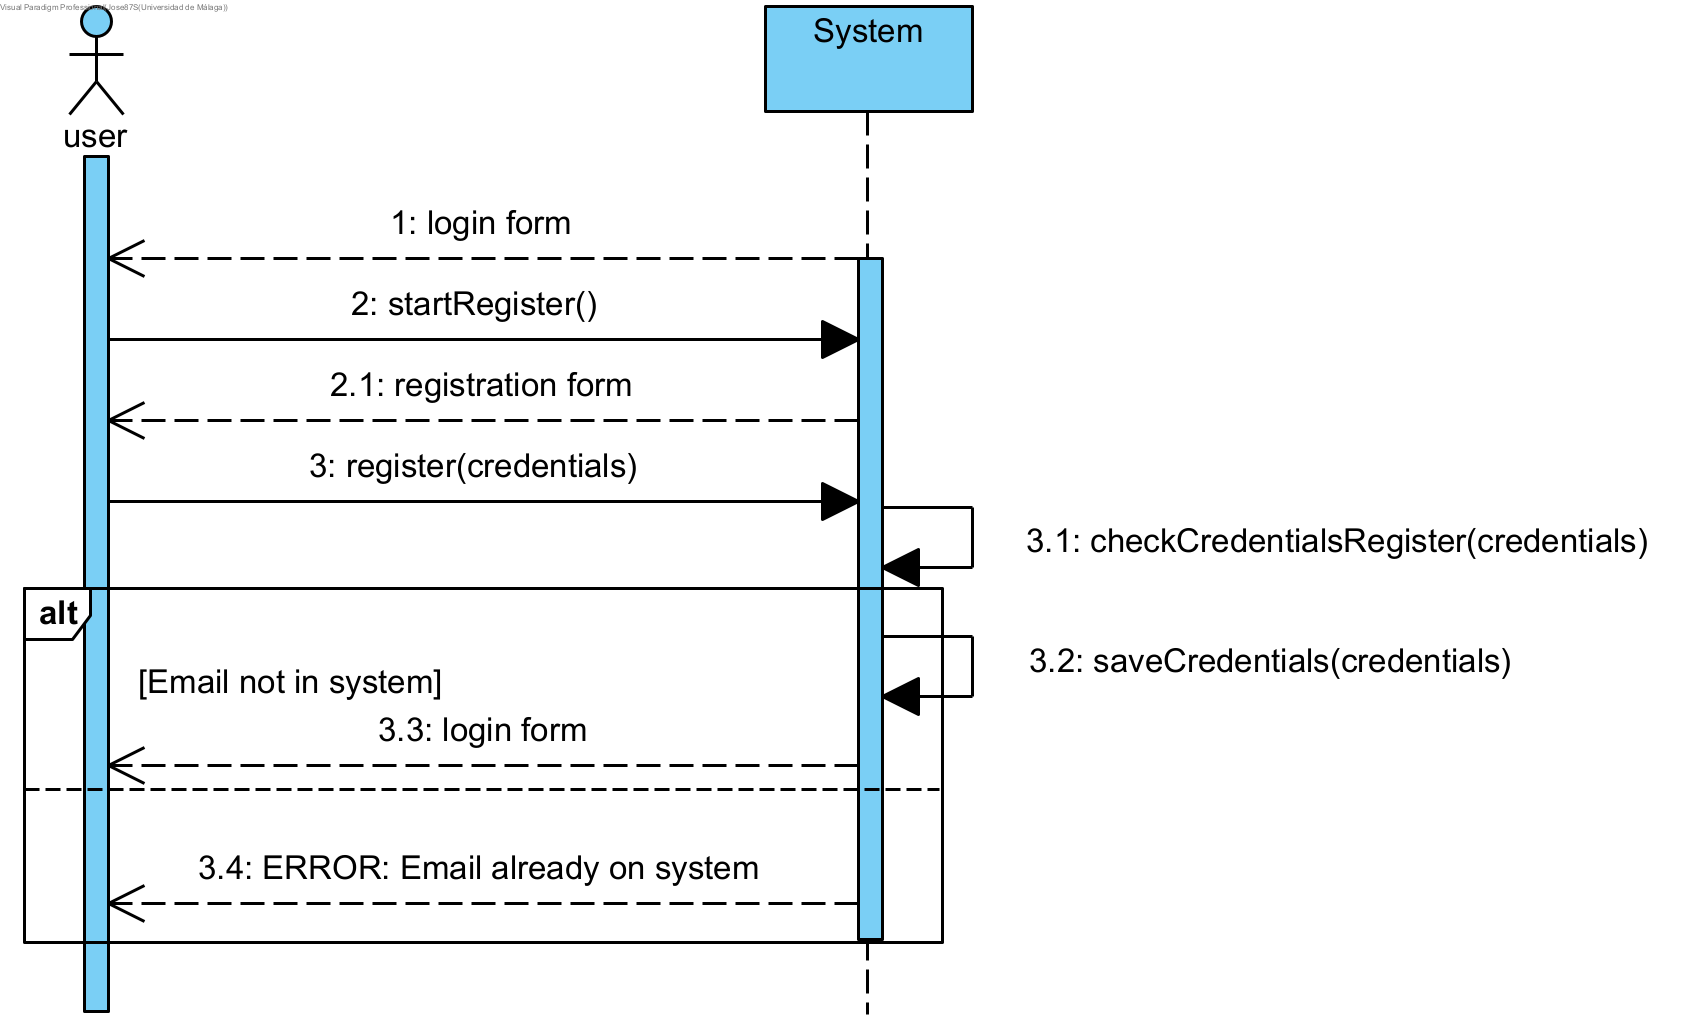
\includegraphics[width=1\textwidth]{images/UseCaseSequenceDiagrams/UC3}
    \caption{Use Case 3}
    \label{fig:UC3}
\end{figure}

\begin{figure}[H]
    \centering
    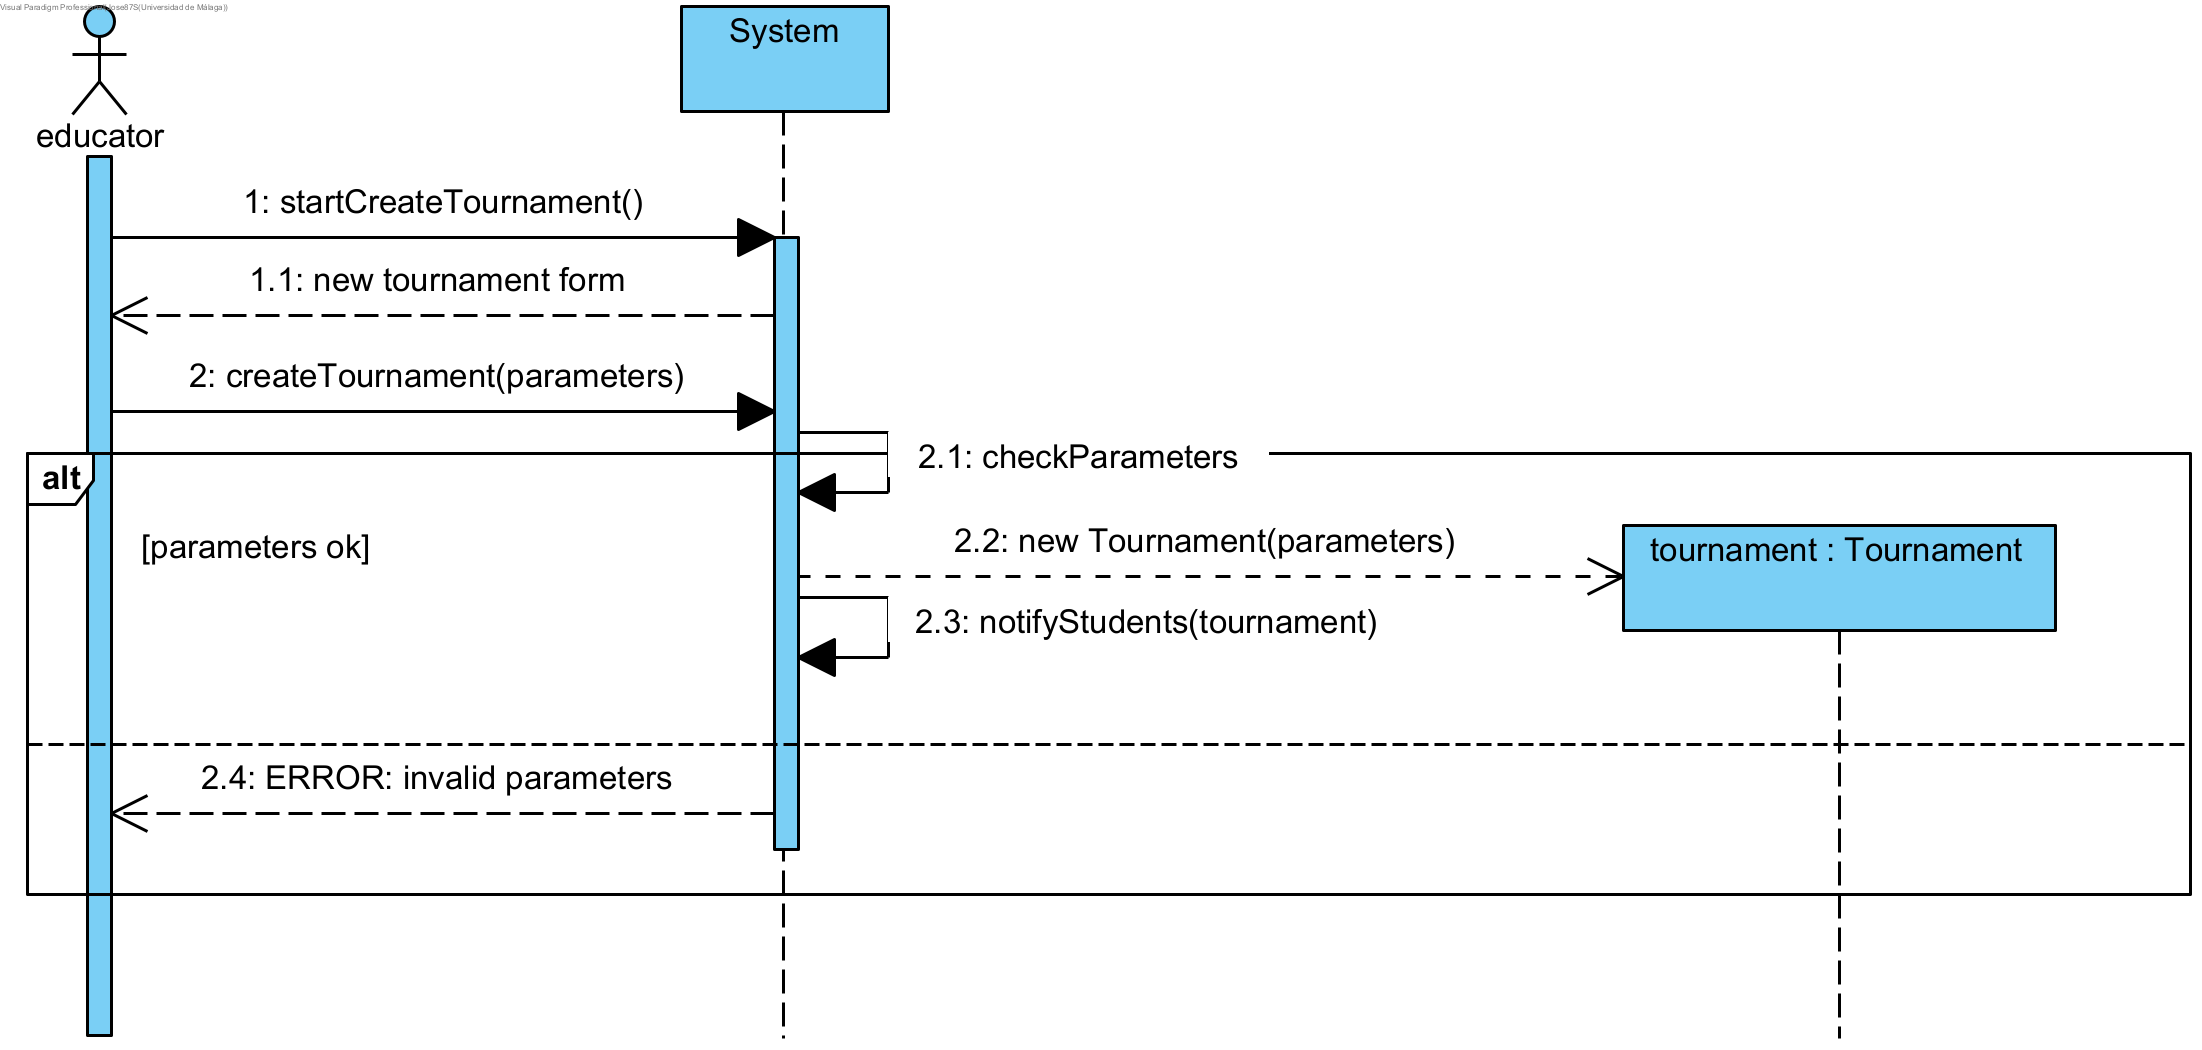
\includegraphics[width=1\textwidth]{images/UseCaseSequenceDiagrams/UC4}
    \caption{Use Case 4}
    \label{fig:UC4}
\end{figure}

\begin{figure}[H]
    \centering
    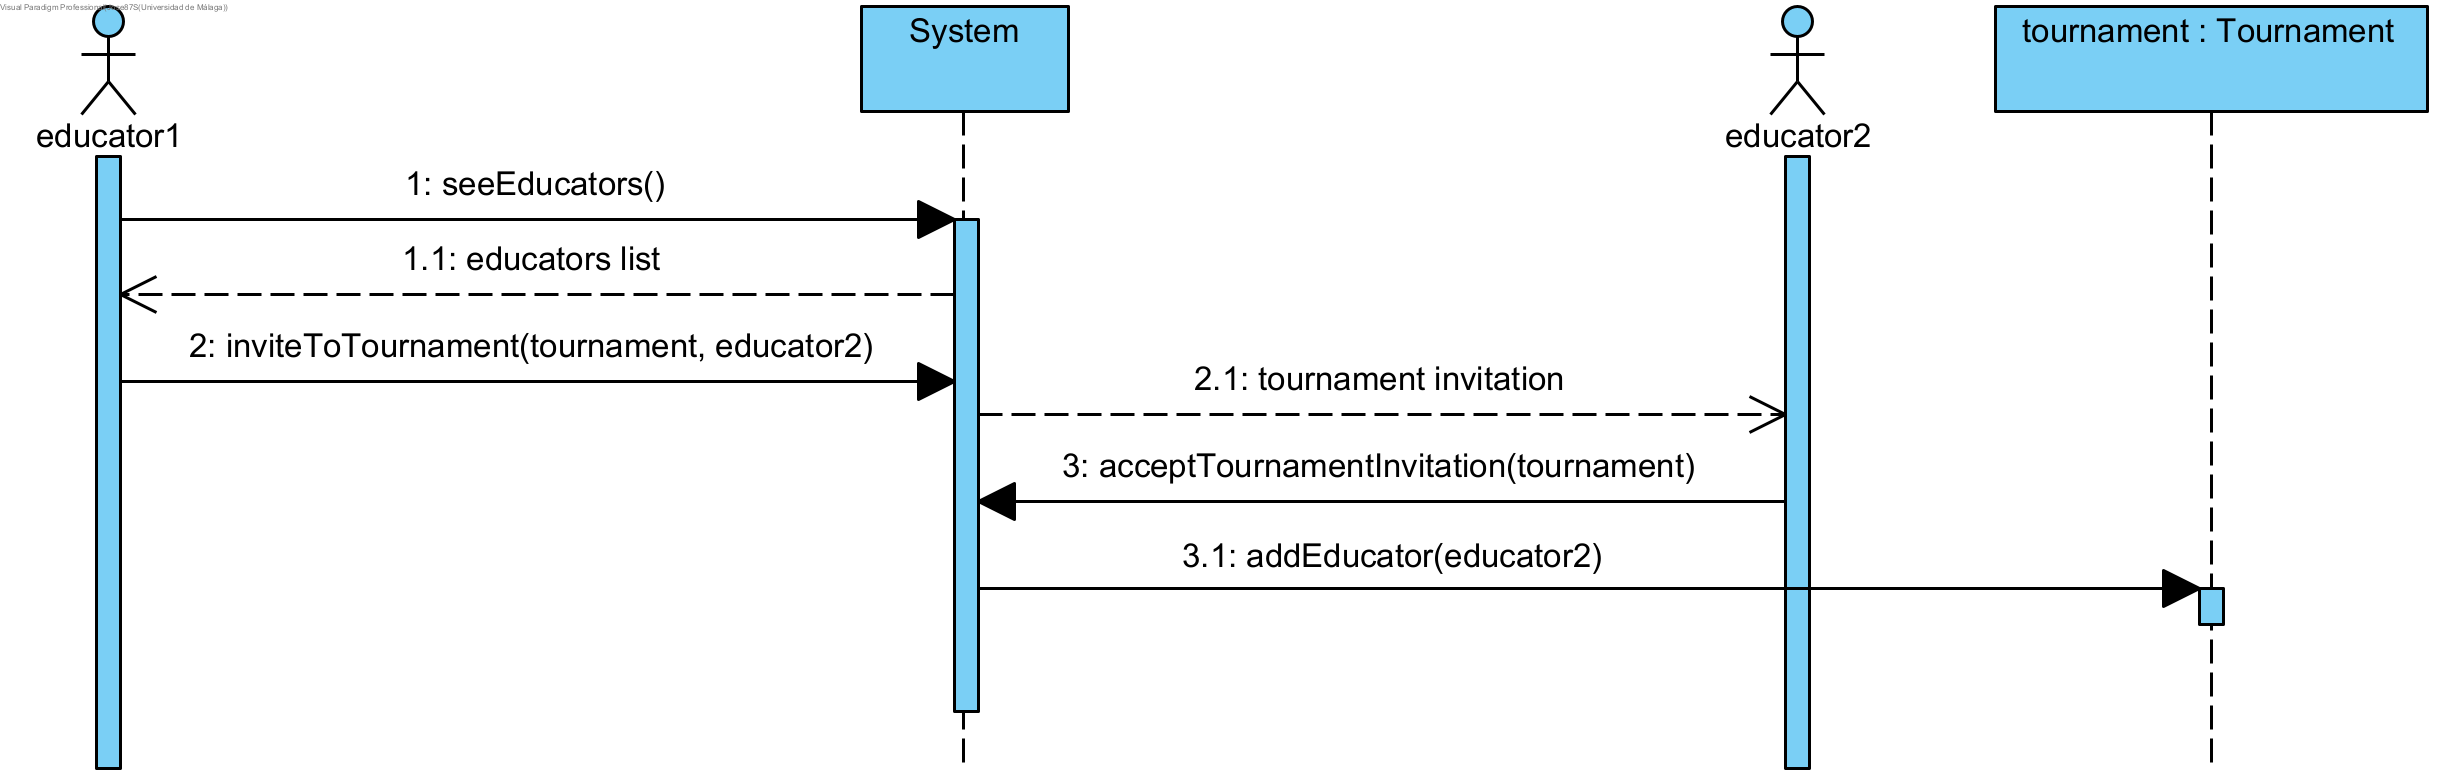
\includegraphics[width=1\textwidth]{images/UseCaseSequenceDiagrams/UC5}
    \caption{Use Case 5}
    \label{fig:UC5}
\end{figure}

\begin{figure}[H]
    \centering
    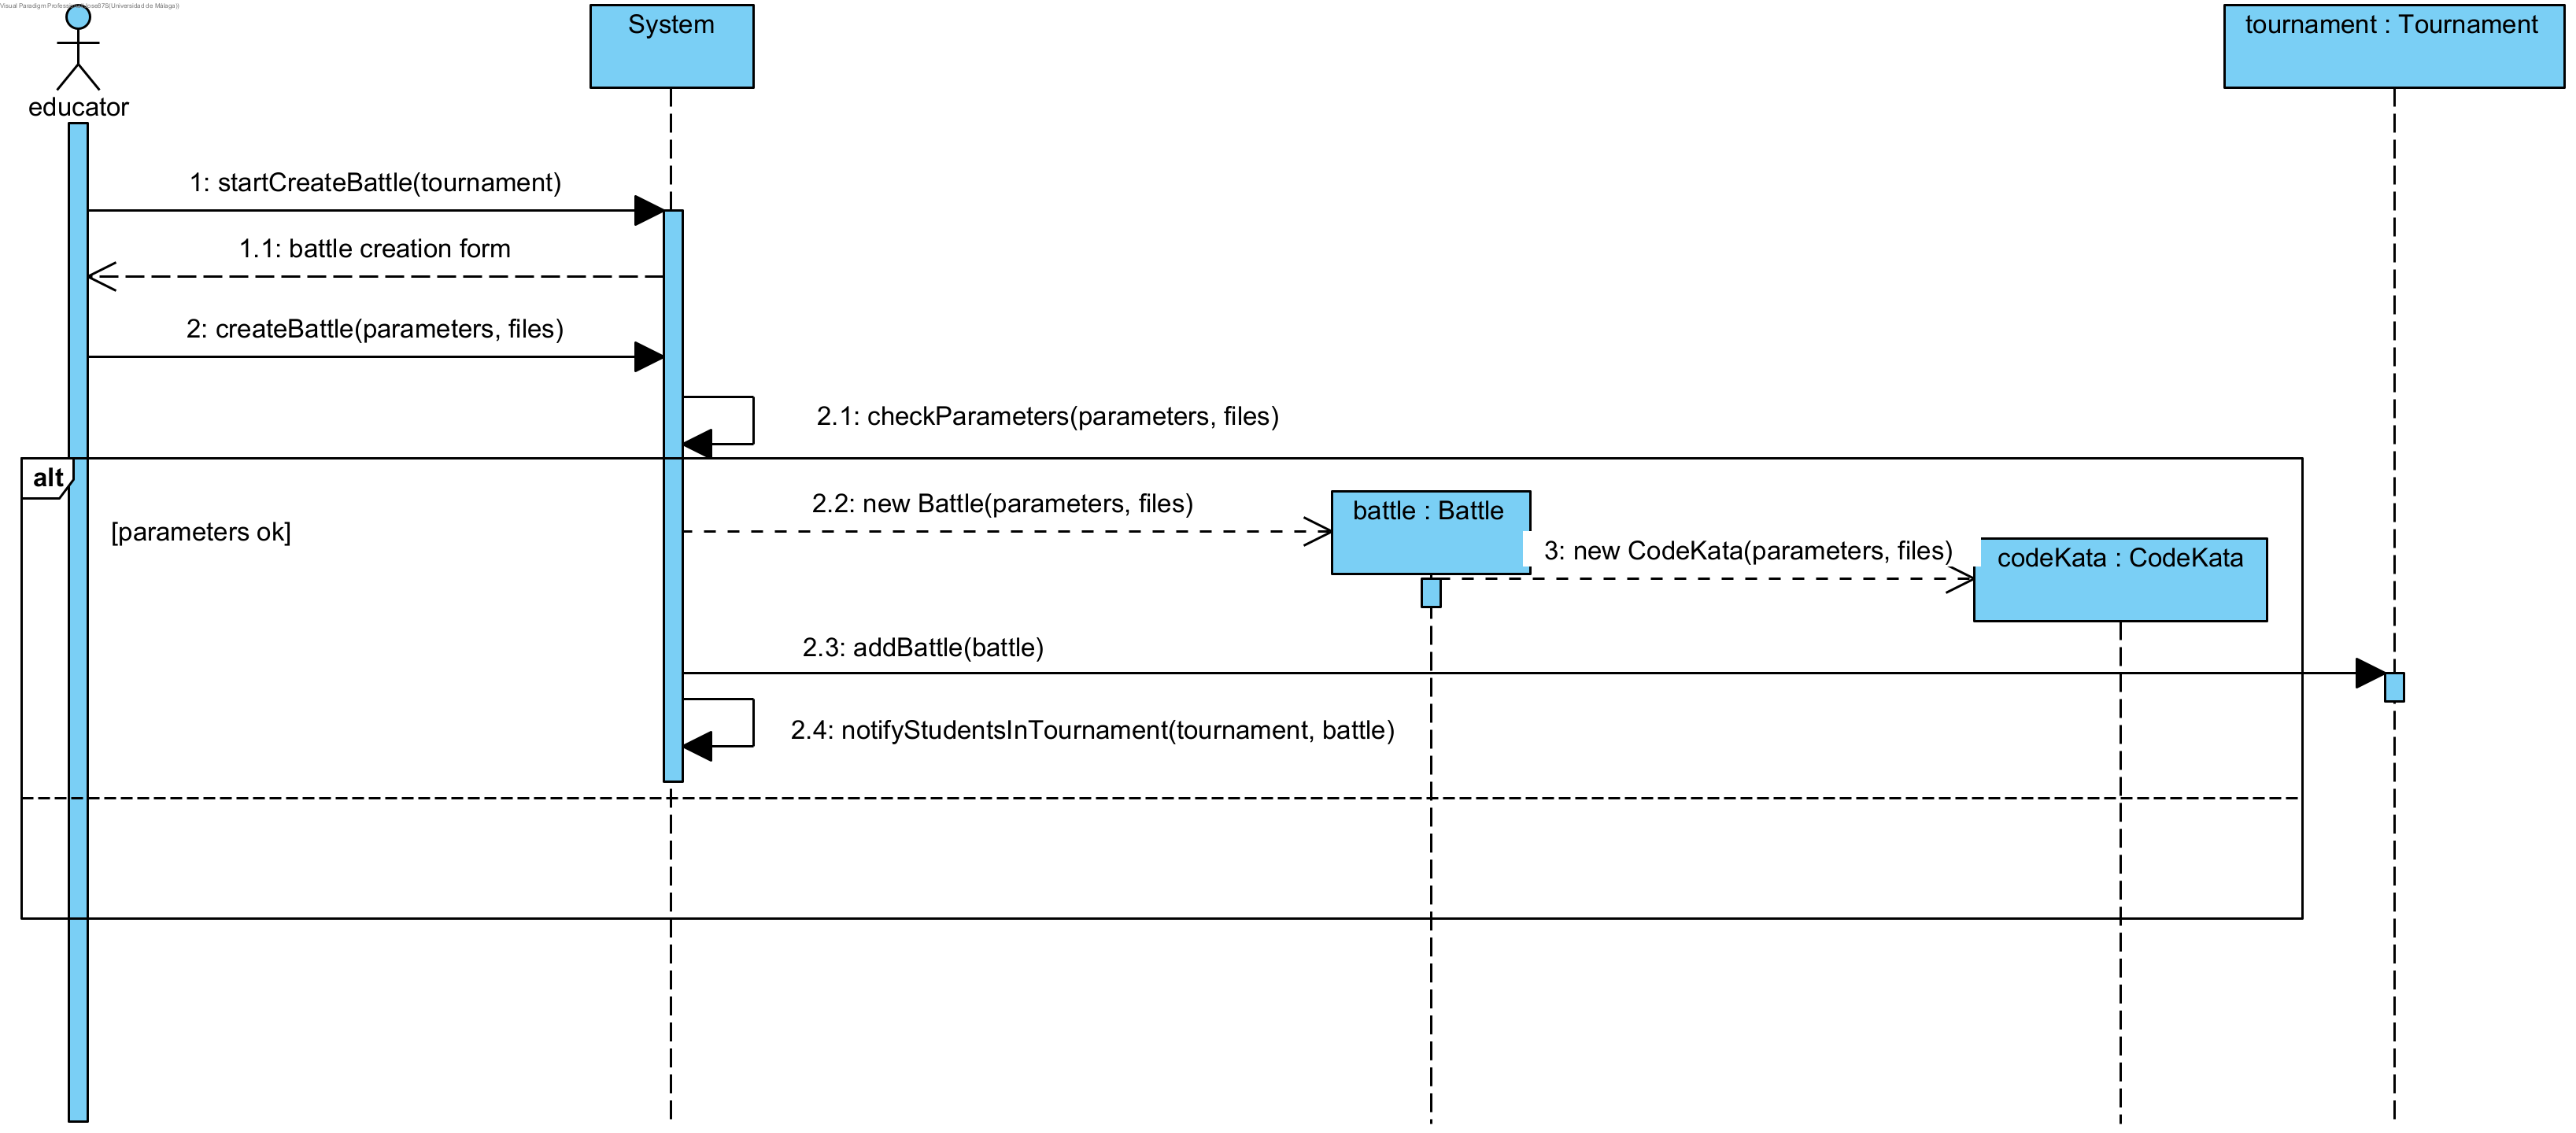
\includegraphics[width=1\textwidth]{images/UseCaseSequenceDiagrams/UC6}
    \caption{Use Case 6}
    \label{fig:UC6}
\end{figure}

\begin{figure}[H]
    \centering
    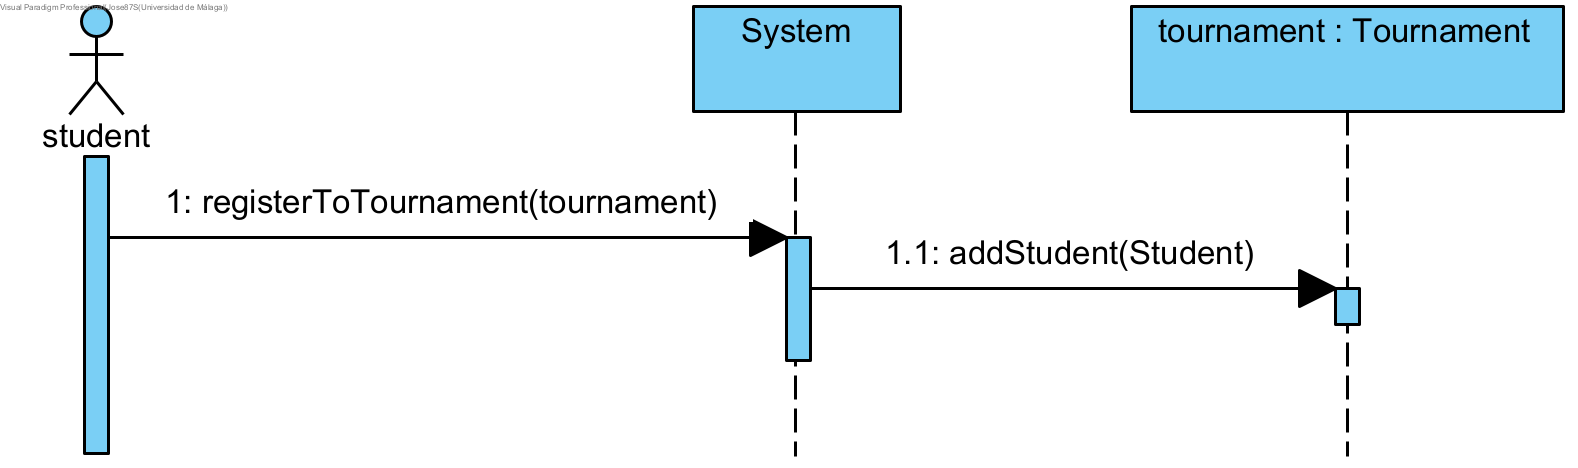
\includegraphics[width=1\textwidth]{images/UseCaseSequenceDiagrams/UC7}
    \caption{Use Case 7}
    \label{fig:UC7}
\end{figure}

\begin{figure}[H]
    \centering
    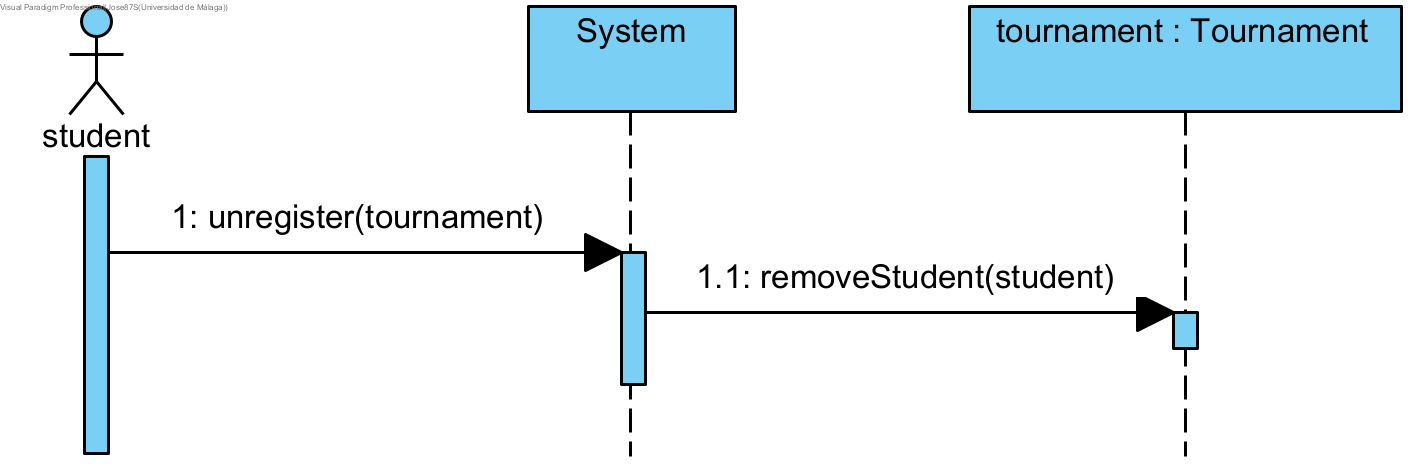
\includegraphics[width=1\textwidth]{images/UseCaseSequenceDiagrams/UC8}
    \caption{Use Case 8}
    \label{fig:UC8}
\end{figure}

\begin{figure}[H]
    \centering
    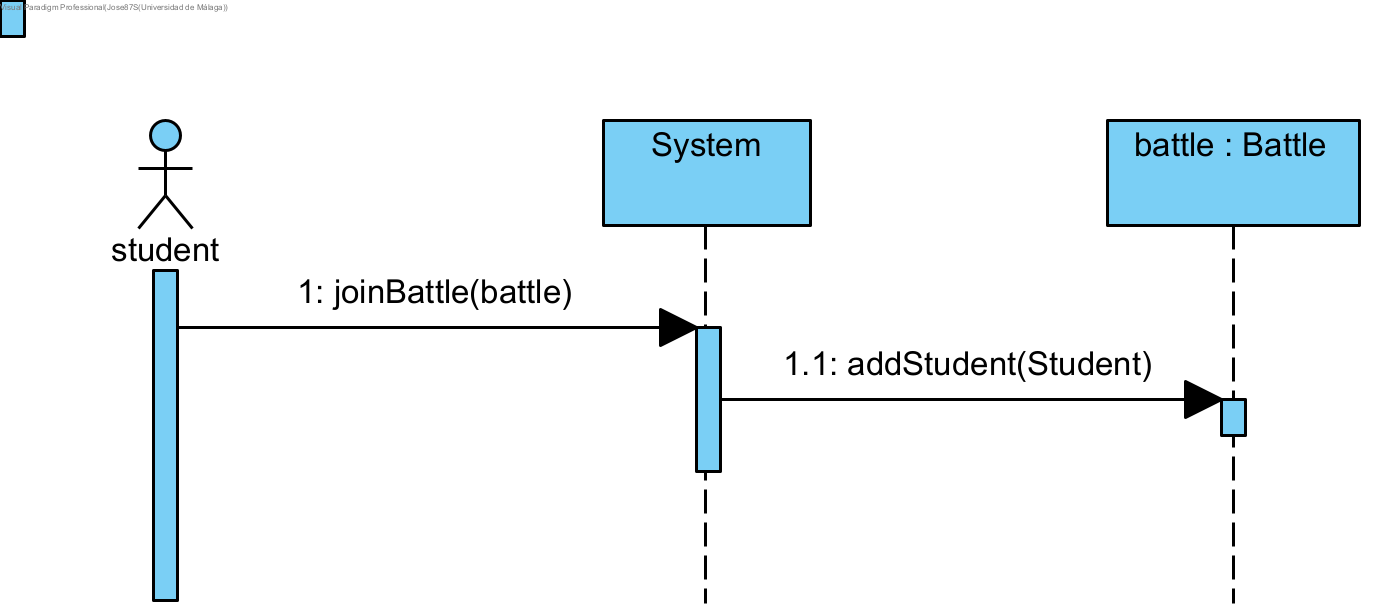
\includegraphics[width=1\textwidth]{images/UseCaseSequenceDiagrams/UC9}
    \caption{Use Case 9}
    \label{fig:UC9}
\end{figure}

\begin{figure}[H]
    \centering
    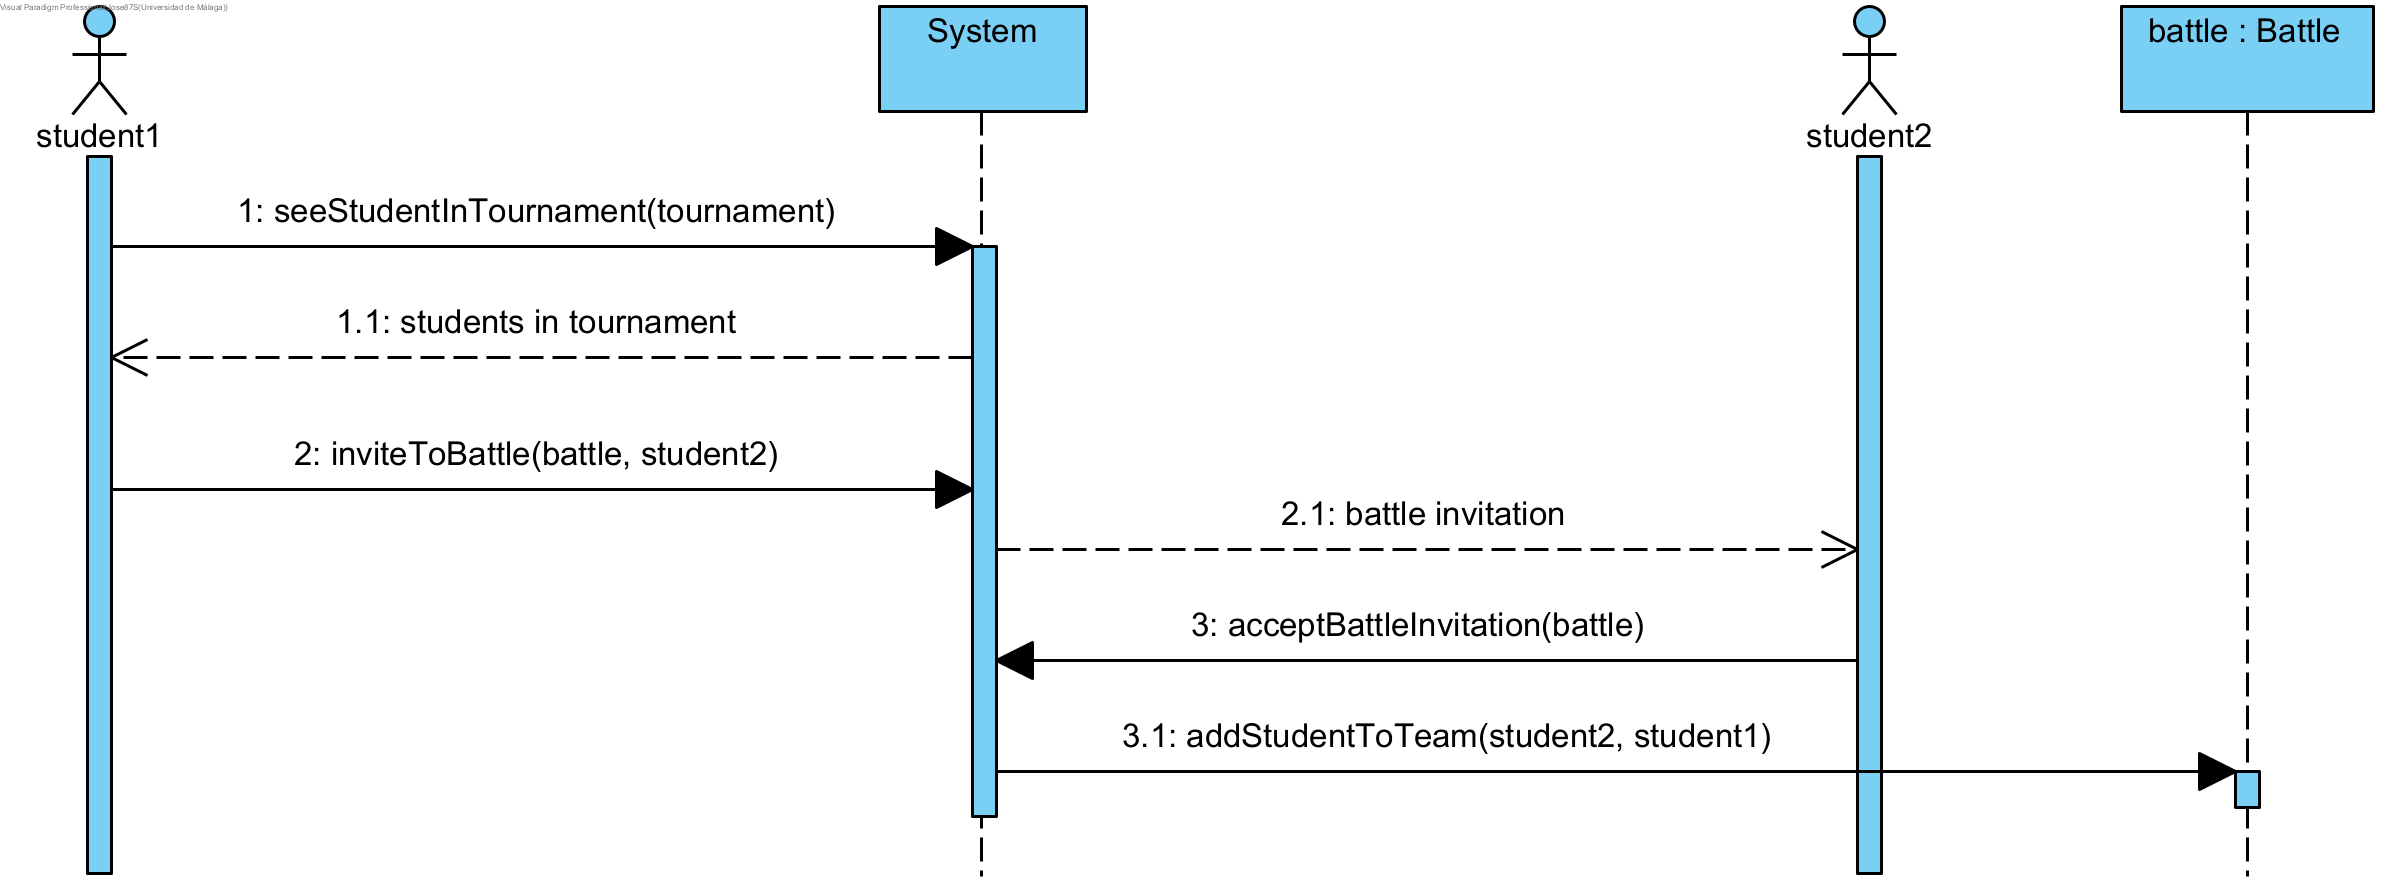
\includegraphics[width=1\textwidth]{images/UseCaseSequenceDiagrams/UC10}
    \caption{Use Case 10}
    \label{fig:UC10}
\end{figure}

\begin{figure}[H]
    \centering
    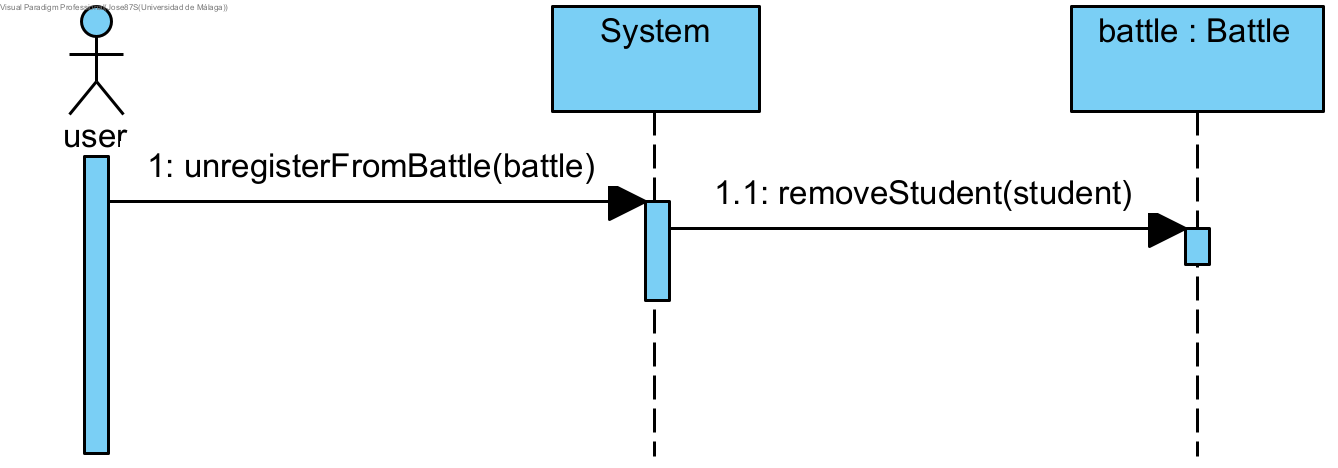
\includegraphics[width=1\textwidth]{images/UseCaseSequenceDiagrams/UC11}
    \caption{Use Case 1}
    \label{fig:UC11}
\end{figure}

\begin{figure}[H]
    \centering
    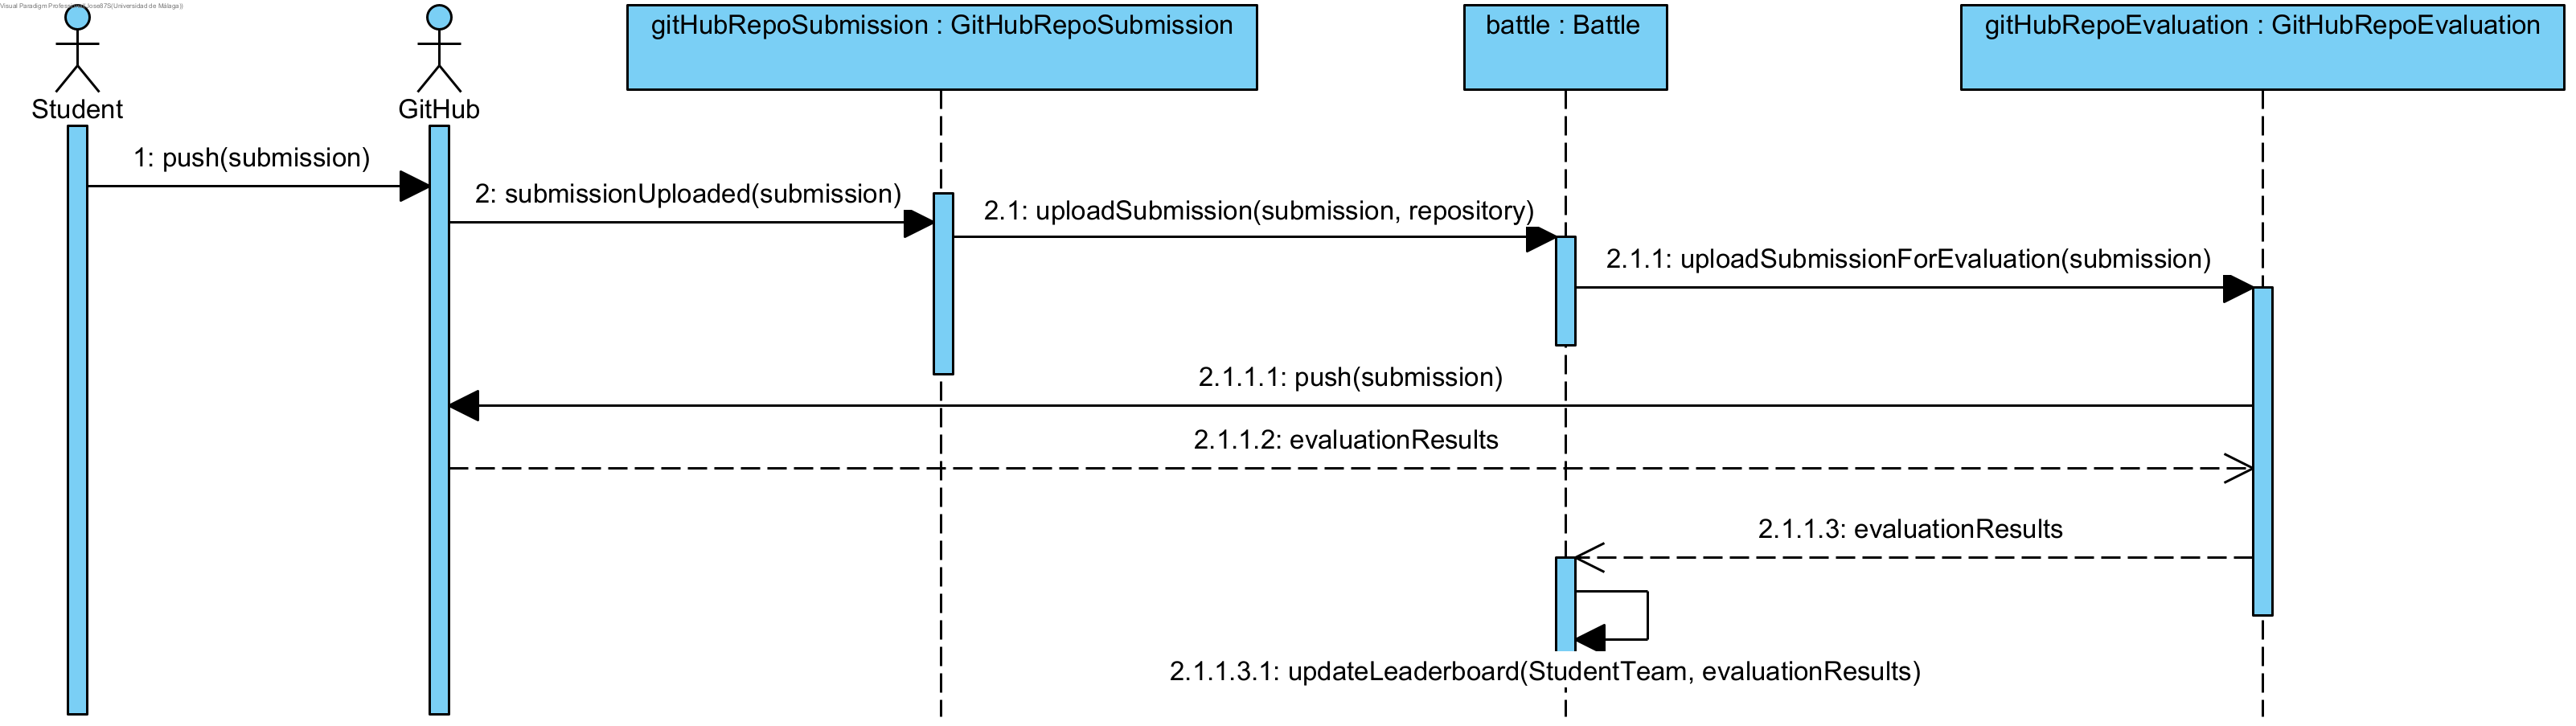
\includegraphics[width=1\textwidth]{images/UseCaseSequenceDiagrams/UC12}
    \caption{Use Case 12}
    \label{fig:UC12}
\end{figure}

\begin{figure}[H]
    \centering
    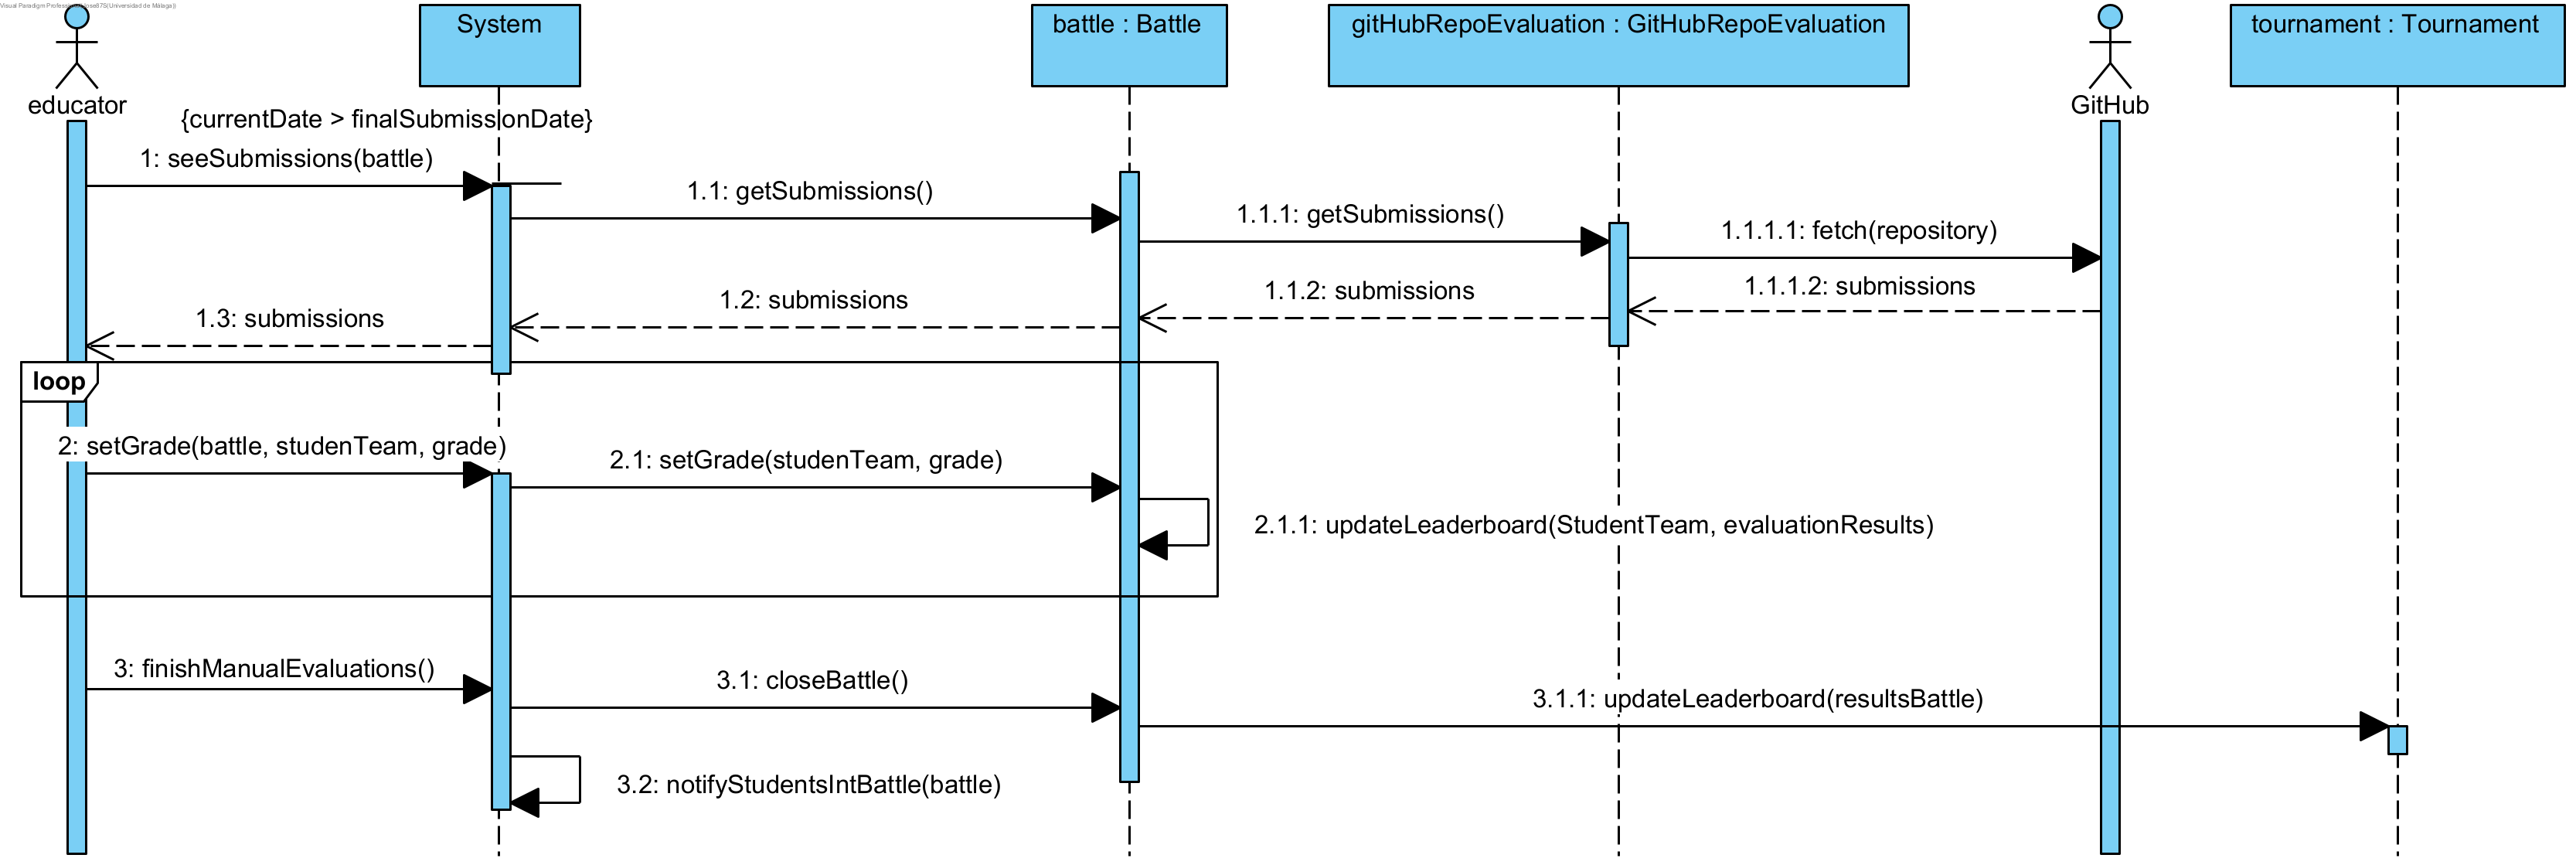
\includegraphics[width=1\textwidth]{images/UseCaseSequenceDiagrams/UC13}
    \caption{Use Case 13}
    \label{fig:UC13}
\end{figure}

\begin{figure}[H]
    \centering
    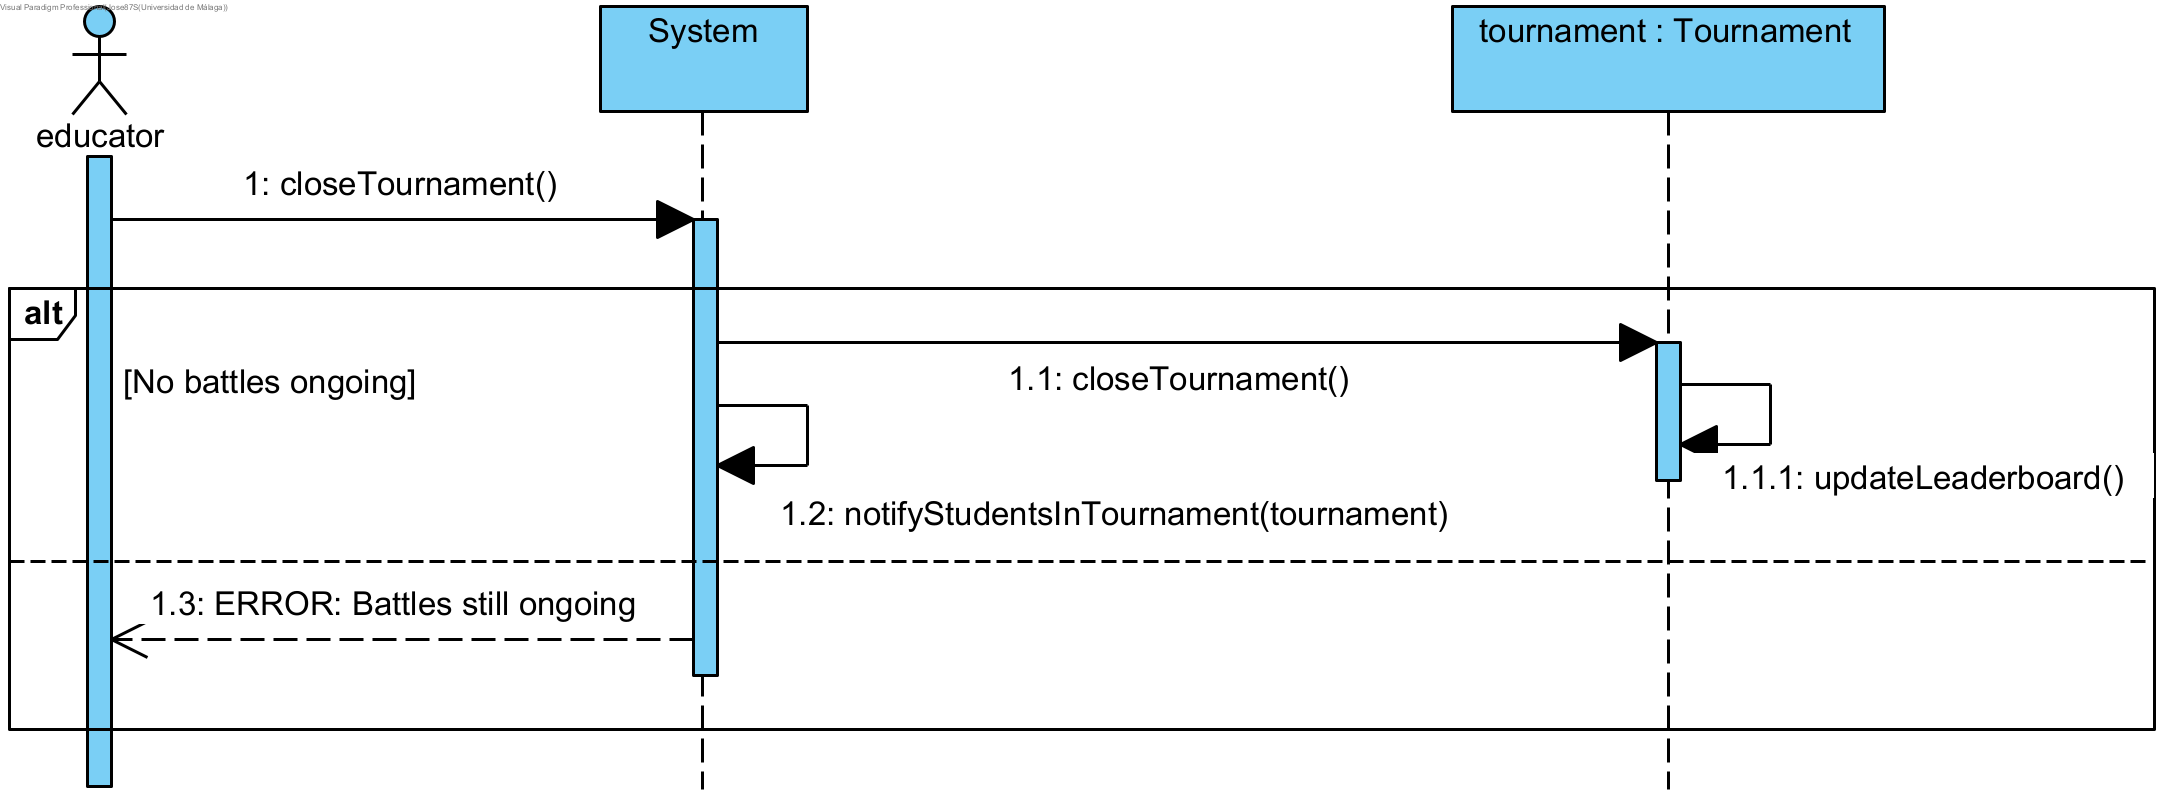
\includegraphics[width=1\textwidth]{images/UseCaseSequenceDiagrams/UC14}
    \caption{Use Case 14}
    \label{fig:UC14}
\end{figure}

\begin{figure}[H]
    \centering
    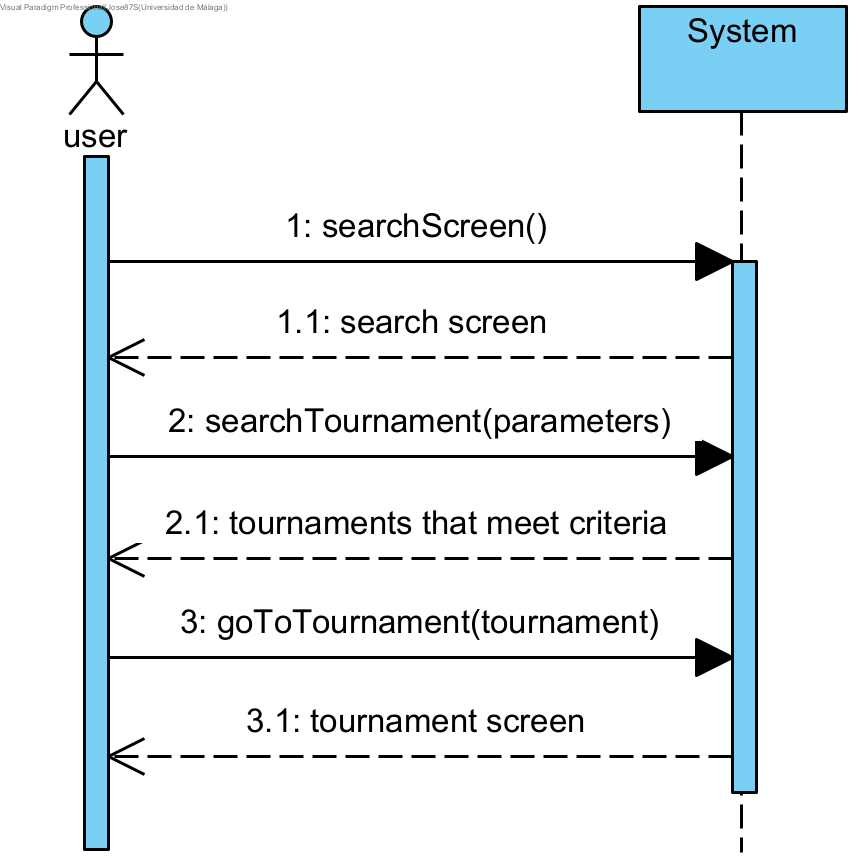
\includegraphics[width=1\textwidth]{images/UseCaseSequenceDiagrams/UC15}
    \caption{Use Case 15}
    \label{fig:UC15}
\end{figure}

\begin{figure}[H]
    \centering
    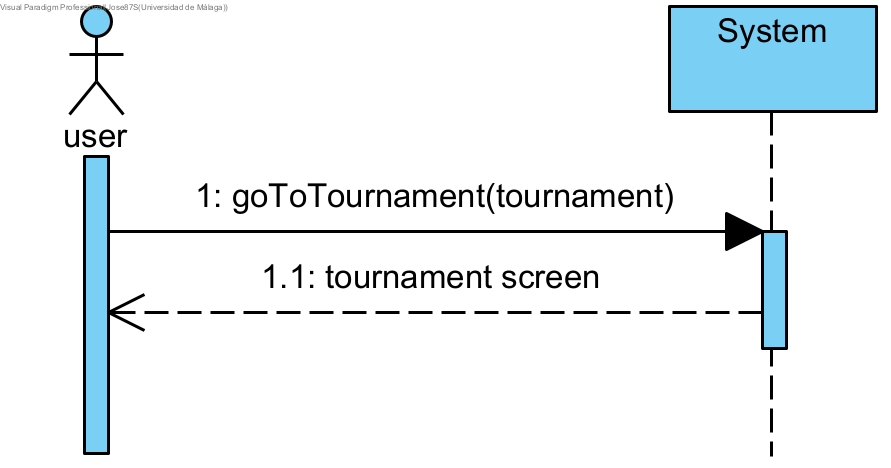
\includegraphics[width=1\textwidth]{images/UseCaseSequenceDiagrams/UC16}
    \caption{Use Case 16}
    \label{fig:UC16}
\end{figure}

\begin{figure}[H]
    \centering
    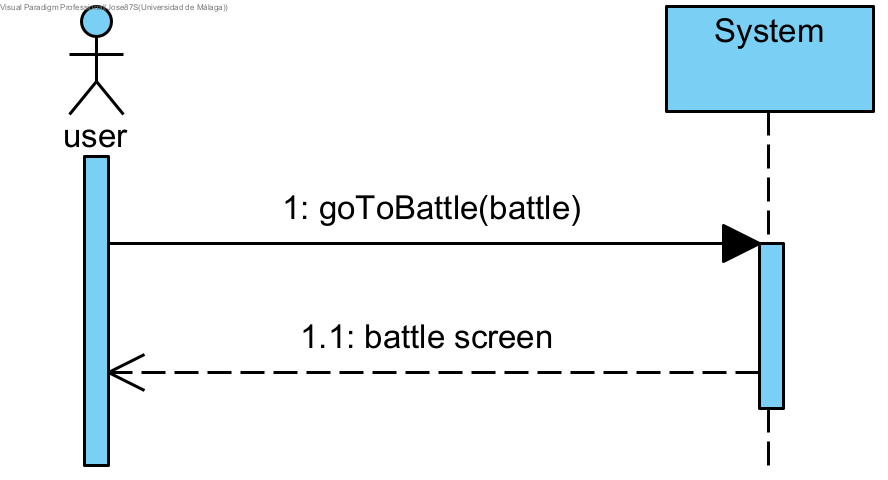
\includegraphics[width=1\textwidth]{images/UseCaseSequenceDiagrams/UC17}
    \caption{Use Case 17}
    \label{fig:UC17}
\end{figure}

\begin{figure}[H]
    \centering
    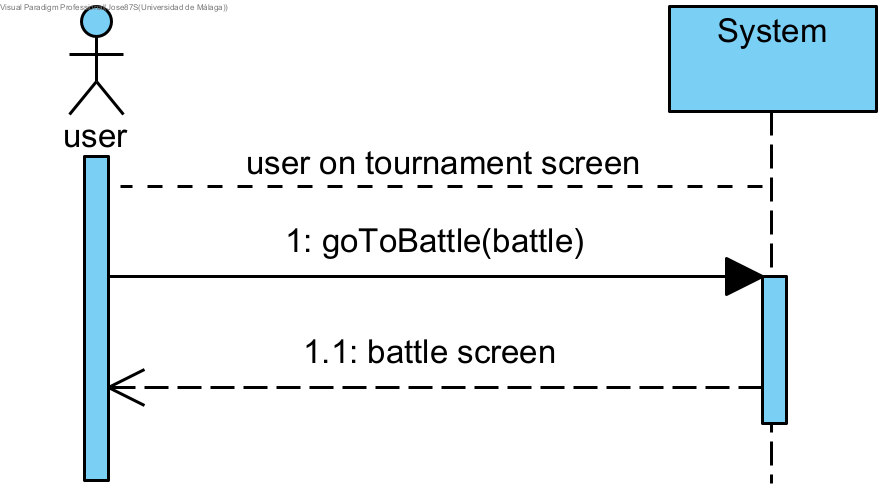
\includegraphics[width=1\textwidth]{images/UseCaseSequenceDiagrams/UC18}
    \caption{Use Case 18}
    \label{fig:UC18}
\end{figure}

\newpage

\subsubsection{Requirements Mapping}

\begin{table}[H]
    \centering
    \begin{tabular*}{\linewidth}{@{\extracolsep{\fill}} cc }
        \hline
        \multicolumn{2}{|c|}{\parbox{0.9\dimexpr\textwidth-2\tabcolsep\relax}{\centering\textbf{G1: Every educator should be able to create a tournament}}} \\
        \hline
        Requirements & R1, R2, R6\\ 
        \hline
        Domain Assumptions & D1\\
        \hline
    \end{tabular*}
\end{table}

\begin{table}[H]
    \centering
    \begin{tabular*}{\linewidth}{@{\extracolsep{\fill}} cc }
        \hline
        \multicolumn{2}{|c|}{\parbox{0.9\dimexpr\textwidth-2\tabcolsep\relax}{\centering\textbf{G2: When creating a tournament, the educator doing so should be able to set a registration deadline and a name.}}} \\
        \hline
        Requirements & R1, R2, R6, R7, R8, R9 \\
        \hline
        Domain Assumptions & D1\\
        \hline
    \end{tabular*}
\end{table}

\begin{table}[H]
    \centering
    \begin{tabular*}{\linewidth}{@{\extracolsep{\fill}} cc }
        \hline
        \multicolumn{2}{|c|}{\parbox{0.9\dimexpr\textwidth-2\tabcolsep\relax}{\centering\textbf{G3: Every educator that owns a tournament should be able to invite other educators to it.}}} \\
        \hline
        Requirements & R1, R2, R6, R11\\
        \hline
        Domain Assumptions & D1\\
        \hline
    \end{tabular*}
\end{table}

\begin{table}[H]
    \centering
    \begin{tabular*}{\linewidth}{@{\extracolsep{\fill}} cc }
        \hline
        \multicolumn{2}{|c|}{\parbox{0.9\dimexpr\textwidth-2\tabcolsep\relax}{\centering\textbf{G4: Every educator that belongs to a tournament should be able to create battles.}}} \\
        \hline
        Requirements & R1, R2, R6, R11, R12\\
        \hline
        Domain Assumptions & D1\\
        \hline
    \end{tabular*}
\end{table}

\begin{table}[H]
    \centering
    \begin{tabular*}{\linewidth}{@{\extracolsep{\fill}} cc }
        \hline
        \multicolumn{2}{|c|}{\parbox{0.9\dimexpr\textwidth-2\tabcolsep\relax}{\centering\textbf{G5: When creating a battle, the educator doing so should be able to set the programming language, a description of the problem, the test cases which will evaluate the students' code, the build automation scripts, the registration deadline, the final submission deadline, the minimum and maximum number of participants per group.}}} \\
        \hline
        Requirements & R1, R2, R6, R11, R12, R13, R14,\\
                     & R15, R16, R17, R18, R19, R20\\
        \hline
        Domain Assumptions & D1, D4, D7\\
        \hline
    \end{tabular*}
\end{table}

\begin{table}[H]
    \centering
    \begin{tabular*}{\linewidth}{@{\extracolsep{\fill}} cc }
        \hline
        \multicolumn{2}{|c|}{\parbox{0.9\dimexpr\textwidth-2\tabcolsep\relax}{\centering\textbf{G6: Every student should be able to see the list of tournaments and register to them before the registration deadline.}}} \\
        \hline
        Requirements & R1, R2, R22, R44\\
        \hline
        Domain Assumptions & D1\\
        \hline
    \end{tabular*}
\end{table}

\begin{table}[H]
    \centering
    \begin{tabular*}{\linewidth}{@{\extracolsep{\fill}} cc }
        \hline
        \multicolumn{2}{|c|}{\parbox{0.9\dimexpr\textwidth-2\tabcolsep\relax}{\centering\textbf{G7: Every student should be able to see the description of the battles of a tournament they belong to and register to them before the registration deadline by themselves or with other students by inviting them to join or by accepting another student's invitation.}}} \\
        \hline
        Requirements & R1, R2, R22, R24, R25, R26, R45, R49\\
        \hline
        Domain Assumptions & D1\\
        \hline
    \end{tabular*}
\end{table}

\begin{table}[H]
    \centering
    \begin{tabular*}{\linewidth}{@{\extracolsep{\fill}} cc }
        \hline
        \multicolumn{2}{|c|}{\parbox{0.9\dimexpr\textwidth-2\tabcolsep\relax}{\centering\textbf{G8: Every time a student makes a submission to a battle, the platform should evaluate it and update the leaderboard of the battle accordingly.}}} \\
        \hline
        Requirements & R1, R2, R22, R24, R30, R31,\\
                     & R32, R33, R34, R35, R36, R37\\
        \hline
        Domain Assumptions & D1, D2, D3, D5, D6\\
        \hline
    \end{tabular*}
\end{table}

\begin{table}[H]
    \centering
    \begin{tabular*}{\linewidth}{@{\extracolsep{\fill}} cc }
        \hline
        \multicolumn{2}{|c|}{\parbox{0.9\dimexpr\textwidth-2\tabcolsep\relax}{\centering\textbf{G9: The evaluation carried out by the platform should be performed with the build automation scripts set by the educator and should be based on the test cases set by the educator and the timeliness of the submission.}}} \\
        \hline
        Requirements & R1, R2, R30, R31, R32, R33,\\
                     & R34, R35, R36, R37\\
        \hline
        Domain Assumptions & D1, D2\\
        \hline
    \end{tabular*}
\end{table}

\begin{table}[H]
    \centering
    \begin{tabular*}{\linewidth}{@{\extracolsep{\fill}} cc }
        \hline
        \multicolumn{2}{|c|}{\parbox{0.9\dimexpr\textwidth-2\tabcolsep\relax}{\centering\textbf{G10: Every student and educator should be able to see the leaderboard of a battle they belong to.}}} \\
        \hline
        Requirements & R1, R2, R29\\
        \hline
        Domain Assumptions & D1\\
        \hline
    \end{tabular*}
\end{table}

\begin{table}[H]
    \centering
    \begin{tabular*}{\linewidth}{@{\extracolsep{\fill}} cc }
        \hline
        \multicolumn{2}{|c|}{\parbox{0.9\dimexpr\textwidth-2\tabcolsep\relax}{\centering\textbf{G11: Once the battle ends, the educator that created it should be able to manually evaluate the code of the students if they so desire to and set a grade for each student.}}} \\
        \hline
        Requirements & R1, R2, R12, R38\\
        \hline
        Domain Assumptions & D1, D8\\
        \hline
    \end{tabular*}
\end{table}

\begin{table}[H]
    \centering
    \begin{tabular*}{\linewidth}{@{\extracolsep{\fill}} cc }
        \hline
        \multicolumn{2}{|c|}{\parbox{0.9\dimexpr\textwidth-2\tabcolsep\relax}{\centering\textbf{G12: Once the educator consolidates the results of a battle, the students that participated in it should be notified and the final results of the battle should be displayed to everyone. The leaderboard of the tournament the battle belongs to should be updated by adding for each student the battle score to the sum of all the other battles they have participated on.
        }}} \\
        \hline
        Requirements & R1, R2, R12, R24, R39, R40, \\
        \hline
        Domain Assumptions & D1\\
        \hline
    \end{tabular*}
\end{table}

\begin{table}[H]
    \centering
    \begin{tabular*}{\linewidth}{@{\extracolsep{\fill}} cc }
        \hline
        \multicolumn{2}{|c|}{\parbox{0.9\dimexpr\textwidth-2\tabcolsep\relax}{\centering\textbf{G13: Every student and educator should be able to see the leaderboard of every tournament.}}} \\
        \hline
        Requirements & R1, R2, R28\\
        \hline
        Domain Assumptions & D1\\
        \hline
    \end{tabular*}
\end{table}

\begin{table}[H]
    \centering
    \begin{tabular*}{\linewidth}{@{\extracolsep{\fill}} cc }
        \hline
        \multicolumn{2}{|c|}{\parbox{0.9\dimexpr\textwidth-2\tabcolsep\relax}{\centering\textbf{G14: An instructor that owns a tournament should be able to close it.}}} \\
        \hline
        Requirements & R1, R2, R6, R41\\
        \hline
        Domain Assumptions & D1\\
        \hline
    \end{tabular*}
\end{table}

\begin{table}[H]
    \centering
    \begin{tabular*}{\linewidth}{@{\extracolsep{\fill}} cc }
        \hline
        \multicolumn{2}{|c|}{\parbox{0.9\dimexpr\textwidth-2\tabcolsep\relax}{\centering\textbf{G15: Once the owner of a tournament closes it, the platform should notify all the students once the leaderboard of the tournament is available.}}} \\
        \hline
        Requirements & R1, R2, R6, R41, R42\\
        \hline
        Domain Assumptions & D1\\
        \hline
    \end{tabular*}
\end{table}

\begin{table}[H]
    \centering
    \begin{tabular*}{\linewidth}{@{\extracolsep{\fill}} cc }
        \hline
        \multicolumn{2}{|c|}{\parbox{0.9\dimexpr\textwidth-2\tabcolsep\relax}{\centering\textbf{G16: When a tournament is created, all students should be notified.}}} \\
        \hline
        Requirements & R1, R2, R6, R10\\
        \hline
        Domain Assumptions & D1\\
        \hline
    \end{tabular*}
\end{table}

\begin{table}[H]
    \centering
    \begin{tabular*}{\linewidth}{@{\extracolsep{\fill}} cc }
        \hline
        \multicolumn{2}{|c|}{\parbox{0.9\dimexpr\textwidth-2\tabcolsep\relax}{\centering\textbf{G17: When a battle is created, all students participating in the tournament the battle belongs to should be notified.}}} \\
        \hline
        Requirements & R1, R2, R12, R21, RR22\\
        \hline
        Domain Assumptions & D1\\
        \hline
    \end{tabular*}
\end{table}

\begin{table}[H]
    \centering
    \begin{tabular*}{\linewidth}{@{\extracolsep{\fill}} cc }
        \hline
        \multicolumn{2}{|c|}{\parbox{0.9\dimexpr\textwidth-2\tabcolsep\relax}{\centering\textbf{G18: A user should be able to browse the platform and find tournaments based on keywords like topics, educators’ names, programming language and experience level.}}} \\
        \hline
        Requirements & R1, R2, R43\\
        \hline
        Domain Assumptions & D1\\
        \hline
    \end{tabular*}
\end{table}

\begin{table}[H]
    \centering
    \begin{tabular*}{\linewidth}{@{\extracolsep{\fill}} cc }
        \hline
        \multicolumn{2}{|c|}{\parbox{0.9\dimexpr\textwidth-2\tabcolsep\relax}{\centering\textbf{G19: A student should be able to cancel their registration to a tournament or battle before the registration deadline.}}} \\
        \hline
        Requirements & R1, R2, R22, R23, R24, R27\\
        \hline
        Domain Assumptions & D1\\
        \hline
    \end{tabular*}
\end{table}


\subsection{Performance Requirements}
\begin{itemize}
  \item \textbf{R50:} The system shall respond to user actions within 1.5 seconds, ensuring a seamless and responsive user experience.
  \item \textbf{R51:} The platform shall support concurrent access by a minimum of 500 users, maintaining optimal performance during peak usage periods.
  \item \textbf{R52:} The system shall handle a database of 100,000 Code Kata problems, ensuring efficient retrieval and storage operations.
\end{itemize}

% Design Constraints
\subsection{Design Constraints}
\subsubsection{Standards Compliance}
\begin{itemize}
  \item \textbf{R53:} The system design shall comply with relevant industry standards for web applications, ensuring compatibility and interoperability.
  \item \textbf{R54:} The user interface design shall adhere to web accessibility standards (WCAG 2.0 or later) to ensure inclusivity for users with disabilities.
\end{itemize}

\subsubsection{Hardware Limitations}
\begin{itemize}
  \item \textbf{R55:} The system shall operate within the hardware specifications outlined in the system requirements documentation, including minimum processor speed, RAM, and storage capacity.
  \item \textbf{R56:} The system shall be compatible with commonly used web browsers, including Chrome, Firefox, Safari, and Edge, ensuring a consistent user experience.
\end{itemize}

\subsubsection{Any Other Constraint}
\begin{itemize}
  \item \textbf{R57:} The system development and deployment shall comply with legal and regulatory requirements, including data protection and privacy laws.
  \item \textbf{R58:} The system shall be designed to accommodate potential variations in user network conditions, such as low bandwidth or intermittent connectivity.
\end{itemize}

% Software System Attributes
\subsection{Software System Attributes}
\subsubsection{Reliability}
\begin{itemize}
  \item \textbf{R59:} The system shall achieve a 99.9\% uptime, minimizing service interruptions and downtime.
  \item \textbf{R60:} The platform shall implement automated data backup procedures to prevent data loss in case of system failures.
\end{itemize}

\subsubsection{Availability}
\begin{itemize}
  \item \textbf{R61:} The system shall be available 24/7, allowing users to access the platform at any time.
  \item \textbf{R62:} The platform shall implement a load balancing mechanism to distribute traffic evenly and ensure optimal availability during peak usage.
\end{itemize}

\subsubsection{Security}
\begin{itemize}
  \item \textbf{R63:} The system shall encrypt user data during transmission to prevent unauthorized access.
  \item \textbf{R64:} The platform shall implement user authentication and authorization mechanisms to control access to sensitive information.
\end{itemize}

\subsubsection{Maintainability}
\begin{itemize}
  \item \textbf{R65:} The system shall provide automated software updates to ensure that the latest features and security patches are applied.
  \item \textbf{R66:} The development team shall document the codebase and provide a user-friendly manual for system administrators.
  \item \textbf{R67:} The development team shall follow patterns and best practices for code organization to ensure that the codebase is easy to maintain and expand.
\end{itemize}

\subsubsection{Portability}
\begin{itemize}
  \item \textbf{R68:} The system shall be compatible with major operating systems, including Windows, macOS, and Linux.
  \item \textbf{R69:} The platform shall support the latest versions of common web browsers to ensure a consistent user experience across different environments.
\end{itemize}

\section{FORMAL ANALYSIS USING ALLOY}
\lstinputlisting[language=alloy]{Alloy/CodeKataBlade.als}

\begin{figure}[H]
    \centering
    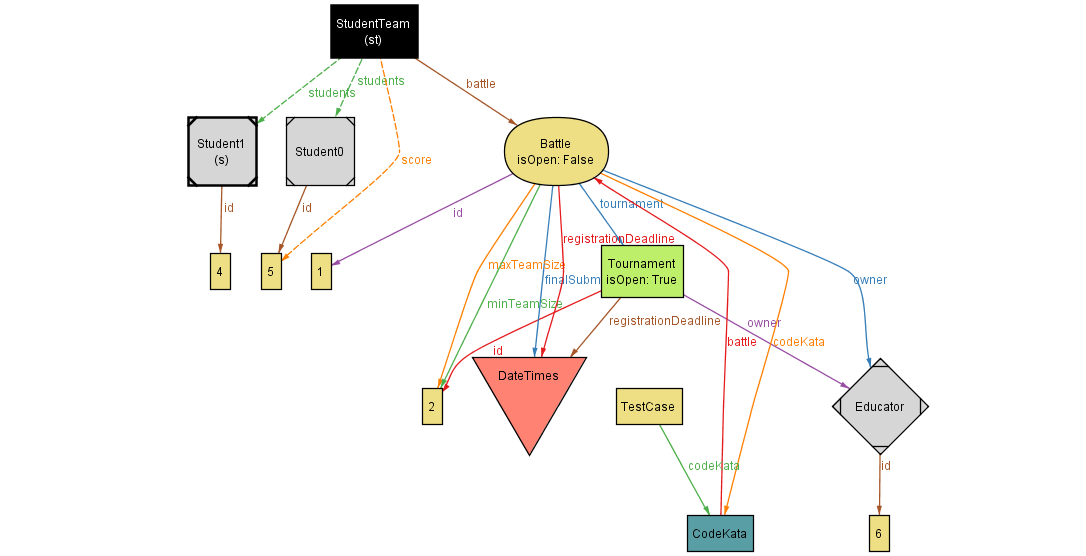
\includegraphics[width=1\textwidth]{Alloy/instance}
    \caption{Alloy Instance}
    \label{fig:AlloyInstance}
\end{figure}

\section{EFFORT SPENT}

\begin{itemize}
    \item Introduction: 4 hours
    \item Overall Description: 10 hours
    \item Specific Requirements: 16 hours
    \item Formal Analysis Using Alloy: 8 hours
\end{itemize}

\section{REFERENCES}

\begin{itemize}
    \item Diagrams done with Visual Paradigm
    \item UI Mockups done with UIzard
    \item GitHub Actions documentation: \url{https://docs.github.com/en/actions}
    \item Alloy documentation: \url{http://alloytools.org/documentation.html}
\end{itemize}


\end{document}

